
% This LaTeX was auto-generated from an M-file by MATLAB.
% To make changes, update the M-file and republish this document.

\documentclass{article}
\usepackage{graphicx}
\usepackage{color}

\sloppy
\definecolor{lightgray}{gray}{0.5}
\setlength{\parindent}{10pt}
\usepackage[margin=1in]{geometry}

\begin{document}

\title{Dynamical Adaptation in ORNs}
\author{Srinivas Gorur-Shandilya}
\maketitle

    
    
\section*{Dynamical Adaptation in ORNs}

\begin{par}
Do ORNs exhibit fast adaptation to a flickering stimulus? Can a simple dynamical adaptation model predict ORN responses to flickering inputs? Here, I take data from Carlotta's random stimulus experiments and first check how well a simple linear prediction from the stimulus compares to the data. Then, I study how the instantaneous gain of the actual ORN response w.r.t to the predicted ORN response varies with time, and try to find a objective filter from the stimulus to this instantaneous gain to correct for systematic errors in the linear prediction.
\end{par} \vspace{1em}

\subsection*{Contents}

\begin{itemize}
\setlength{\itemsep}{-1ex}
   \item Data Visualisation
   \item Filter Extraction
   \item Analysis of Linear Prediction - Which input predicts output better?
   \item Analysis of Linear Prediction - Linearity of Prediction
   \item Analysis of Linear Prediction - Response to High and Low Stimuli
   \item Analysis of Linear Prediction - Filter Variation
   \item Analysis of Gain: Instantaneous Gain and Fitted Gain
   \item Analysis of Gain: Smoothed gain.
   \item Gain Analysis - Estimating the gain
   \item Re-evaluating filter performance after filtering ORN responses
   \item A note on elastic net regularisation
   \item Next Steps
   \item Docs
   \item MATLAB� Code
\end{itemize}


\subsection*{Data Visualisation}

\begin{par}
Data from this file will be used for this analysis.
\end{par} \vspace{1em}

        \color{lightgray} \begin{verbatim}/data/random-stim/final_2011_06_14_ab3A_1o3ol3X-3_20ml_30sec_30ms_rand.mat
\end{verbatim} \color{black}
    \begin{par}
Here, data from simultaneous measurements of the stimulus and from the ORN is shown. The top row shows the valve command signal (a binary signal, high means valve is open). The middle row shows the simultaneous measurement of the odour stimulus with a PID, and the bottom row shows the instantaneous firing rate of the ORN recorded from. In blue is the data computed using Carlotta's code from the raw data. In red is the data computed using my code. Notably different is the firing rate curve, which is much smoother and loses all the high-frequency wiggles. This is because I use a Gaussian smoothing window to do this, while Carlotta uses a boxcar window.
\end{par} \vspace{1em}

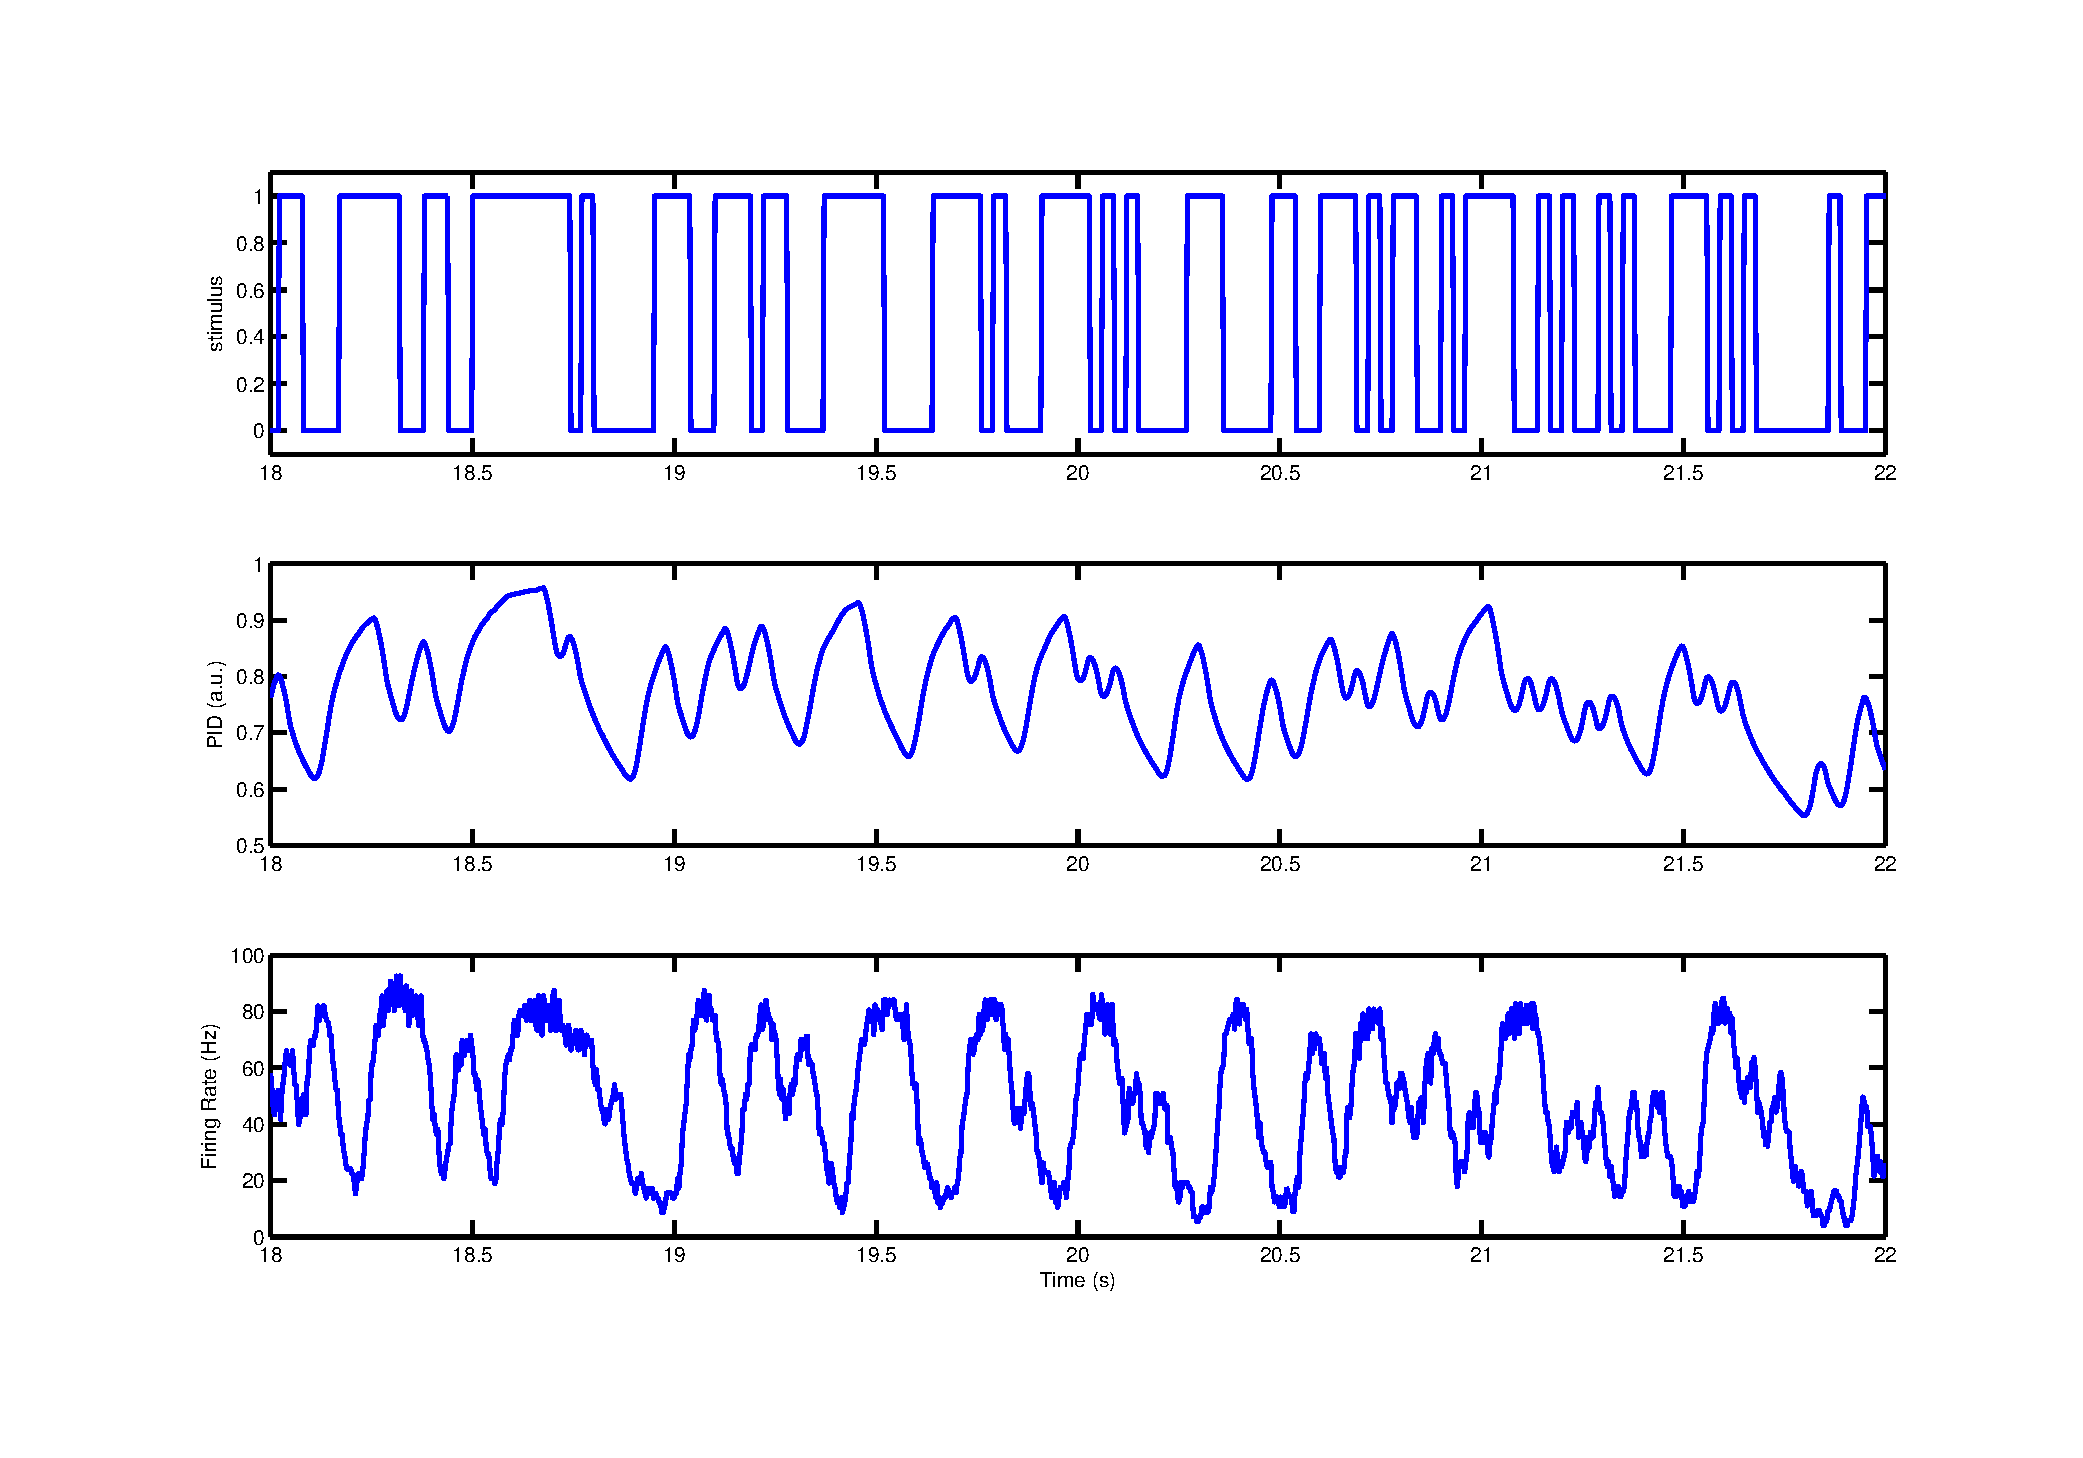
\includegraphics [width=\textwidth]{Analysis_January_01.pdf}
\begin{par}
The odour used, the neuron recorded from and the correlation time of the flickering stimulus are in the file name displayed above the plot.
\end{par} \vspace{1em}


\subsection*{Filter Extraction}

\begin{par}
Details about the filter extraction, regularisation methods, and validation with synthetic and real data is listed in (FilterExtraction.pdf). Here, we calculate the best filter (scaled to ensure that gain = 1) using techniques described in that document from the PID (left) and from the Valve (right).
\end{par} \vspace{1em}

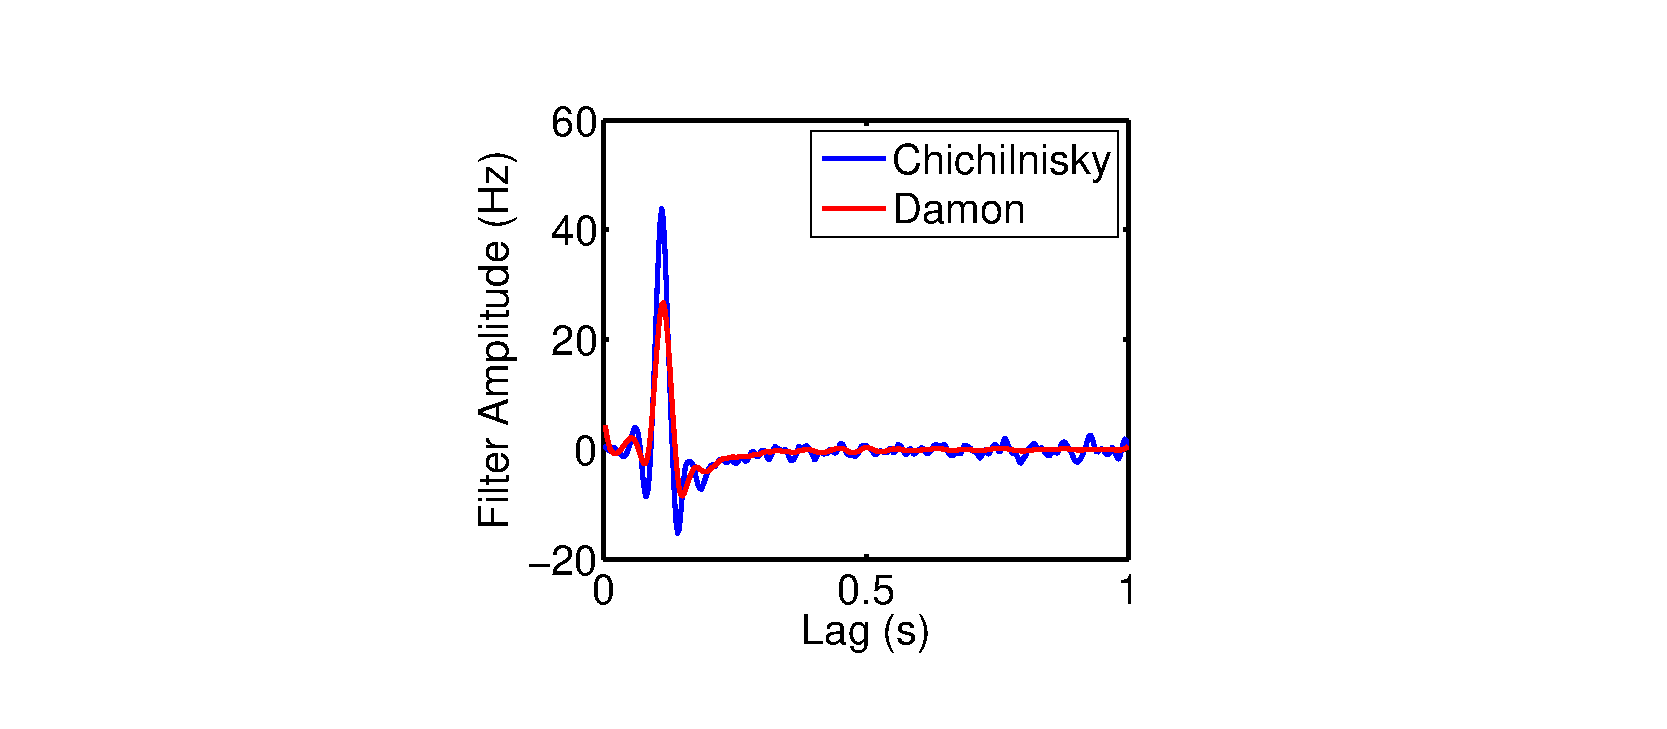
\includegraphics [width=\textwidth]{Analysis_January_02.pdf}
\begin{par}
The variation of filter shape with regularisation parameter for the PID \ensuremath{>} f filter is shown below:
\end{par} \vspace{1em}

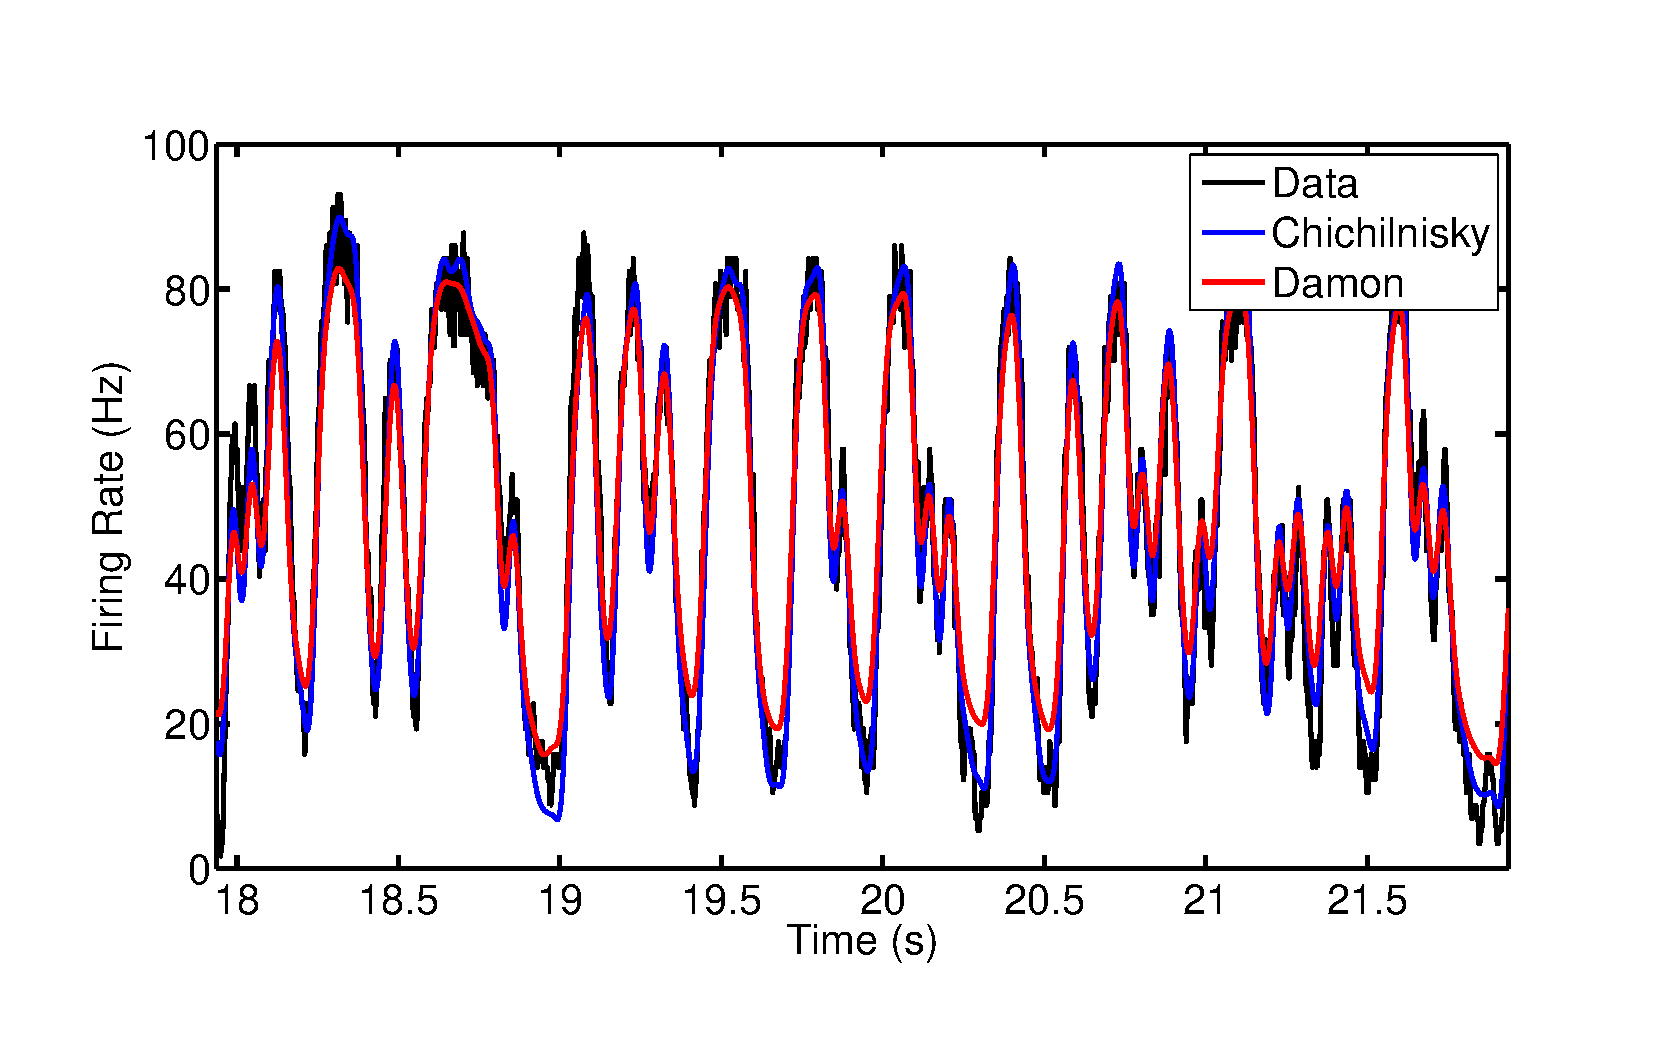
\includegraphics [width=\textwidth]{Analysis_January_03.pdf}
\begin{par}
The variation of filter shape with regularisation parameter for the Valve \ensuremath{>} f filter is shown below:
\end{par} \vspace{1em}

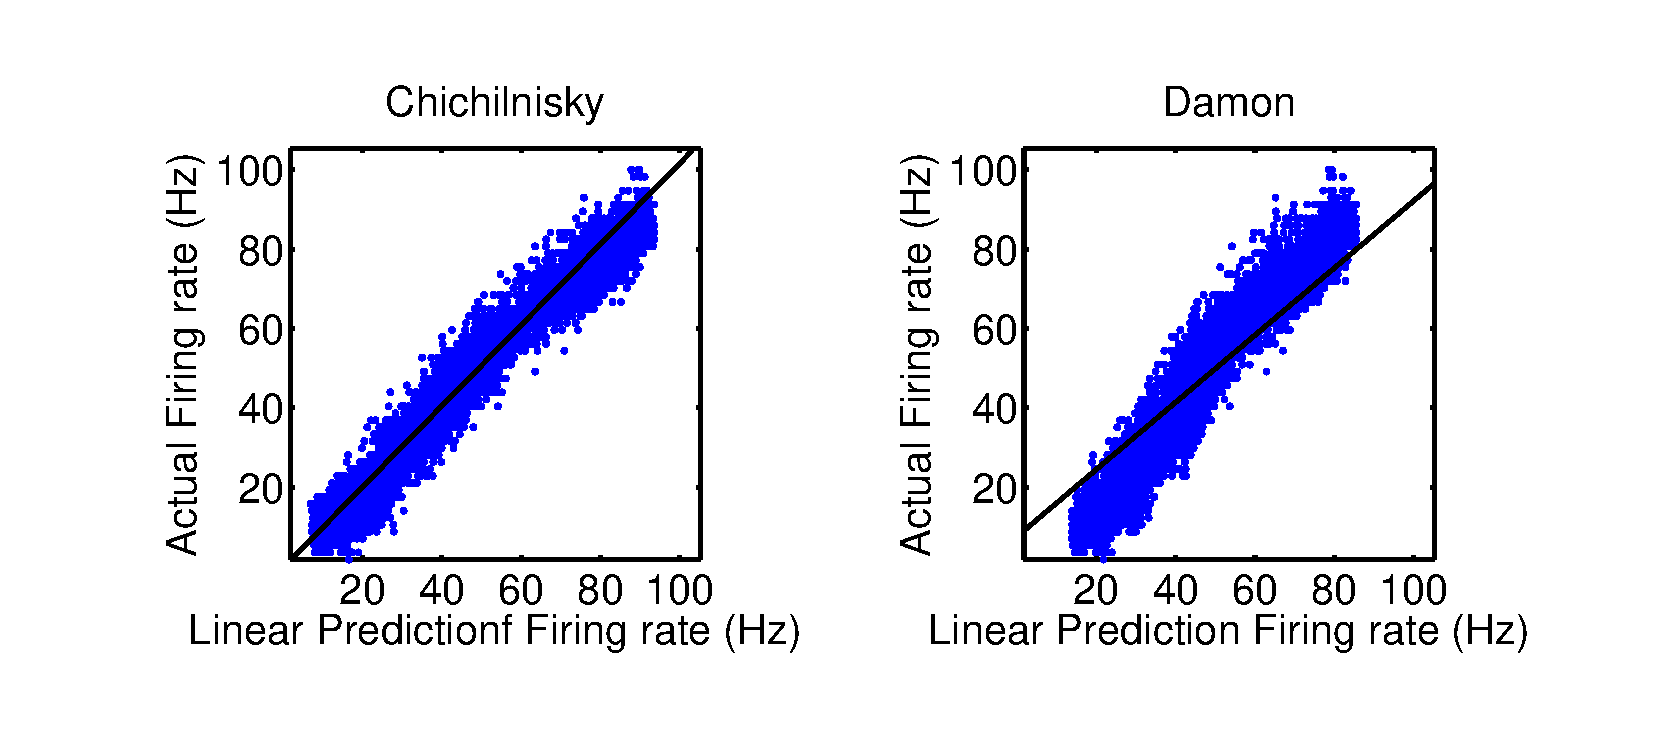
\includegraphics [width=\textwidth]{Analysis_January_04.pdf}
\begin{par}
The convolution of this filter with the input (PID) gives a prediction of the output. In the figure below, the data is shown in black, and the prediction from the PID filter is shown in blue and the prediction from the Valve filter is shown in red. Note that sometimes the prediction can be below zero, which doesn't mean anything physical (firing rate cannot be \ensuremath{<} 0).
\end{par} \vspace{1em}

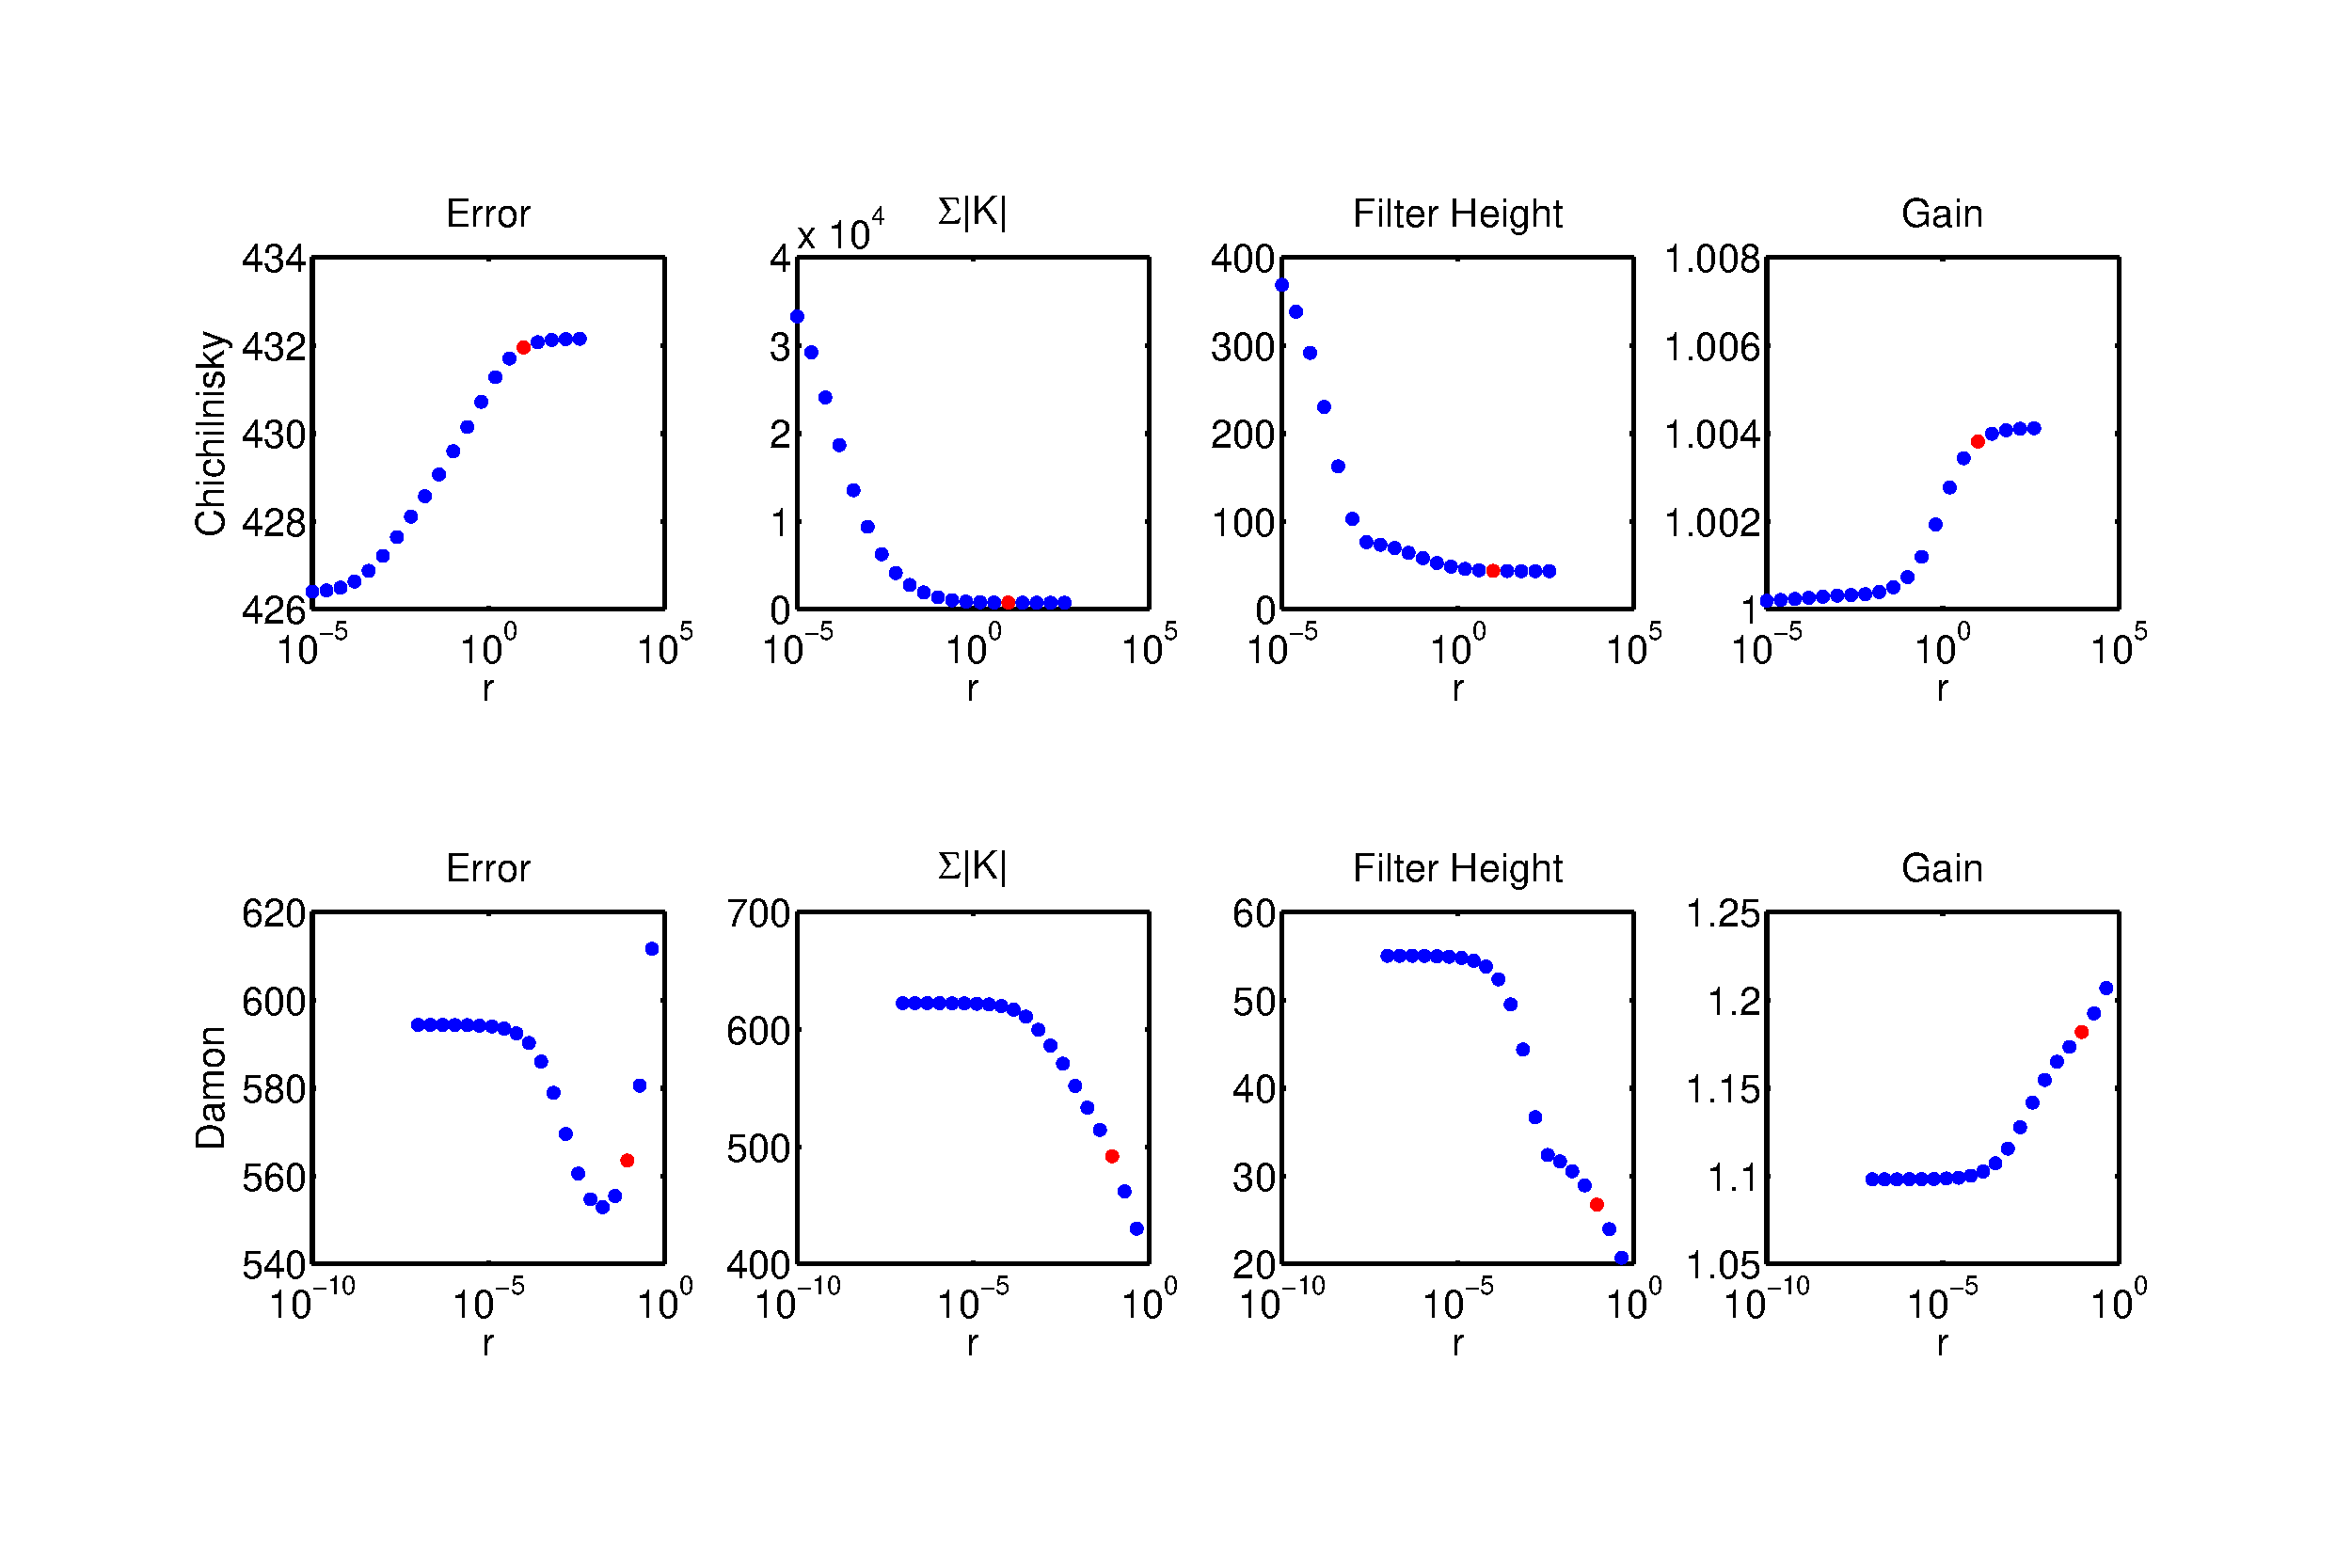
\includegraphics [width=\textwidth]{Analysis_January_05.pdf}


\subsection*{Analysis of Linear Prediction - Which input predicts output better?}

\begin{par}
The measurement of the stimulus should help us predict the response of the neuron better than just the valve control signal, as we now capture the fast fluctuations of the odour stimulus as it reaches the ORN. Thus, a prediction of ORN firing response from the PID signal should be better than a prediction of the ORN firing response from the valve signal.
\end{par} \vspace{1em}
\begin{par}
The r-square (coefficient of determination) of the PID\ensuremath{>}f prediction is:
\end{par} \vspace{1em}

        \color{lightgray} \begin{verbatim}    0.9592

\end{verbatim} \color{black}
    \begin{par}
The r-square (coefficient of determination) of the Valve\ensuremath{>}f prediction is:
\end{par} \vspace{1em}

        \color{lightgray} \begin{verbatim}    0.9599

\end{verbatim} \color{black}
    

\subsection*{Analysis of Linear Prediction - Linearity of Prediction}

\begin{par}
For a linear filter calculated from the data, a plot of the actual response to the predicted response can be fit with a line of slope 1. Here the actual firing rate is plotted on the X axis and the firing rate predicted from the linear filter is plotted on the Y axis.
\end{par} \vspace{1em}

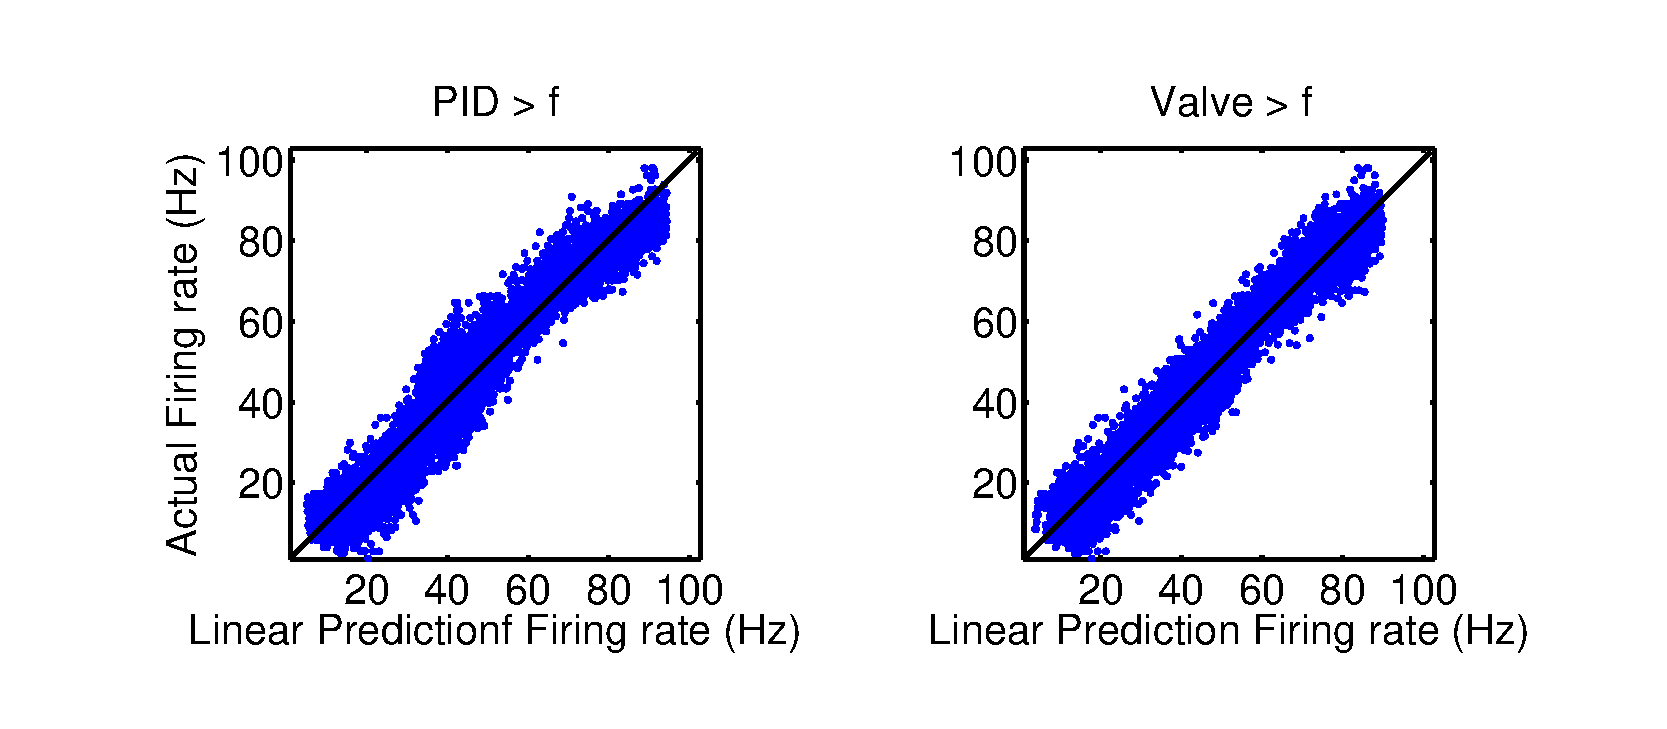
\includegraphics [width=\textwidth]{Analysis_January_06.pdf}
\begin{par}
The lines are best fits to all the data. The slopes of these lines should be exactly 1 as the "best filters" are supposed to be unit gain. The slope, in fact is:
\end{par} \vspace{1em}

        \color{lightgray} \begin{verbatim}    1.0000

\end{verbatim} \color{black}
    

\subsection*{Analysis of Linear Prediction - Response to High and Low Stimuli}

\begin{par}
How does the response of the ORN differ for high and low stimuli? Specifically, does the neuron display the characteristics of fast adaptation to this flickering stimulus?
\end{par} \vspace{1em}
\begin{par}
To look at this, we calculate the mean average stimulus over some window history length for every time point \textit{t}, for various different window history lengths. The effect of this operation is shown in the figure below, where the legend refers to the history window in ms.
\end{par} \vspace{1em}
\begin{par}
To calcualte the mean average stimulus, I use the \textit{filtfilt} function, which is a zero-phase digital filter that works by passing it through once in the forward direction, and once again in the reverse direction. I previously used the simple \textit{filter} function, but the results are substantially different: now, the separation of gains extends for larger history window lengths.
\end{par} \vspace{1em}

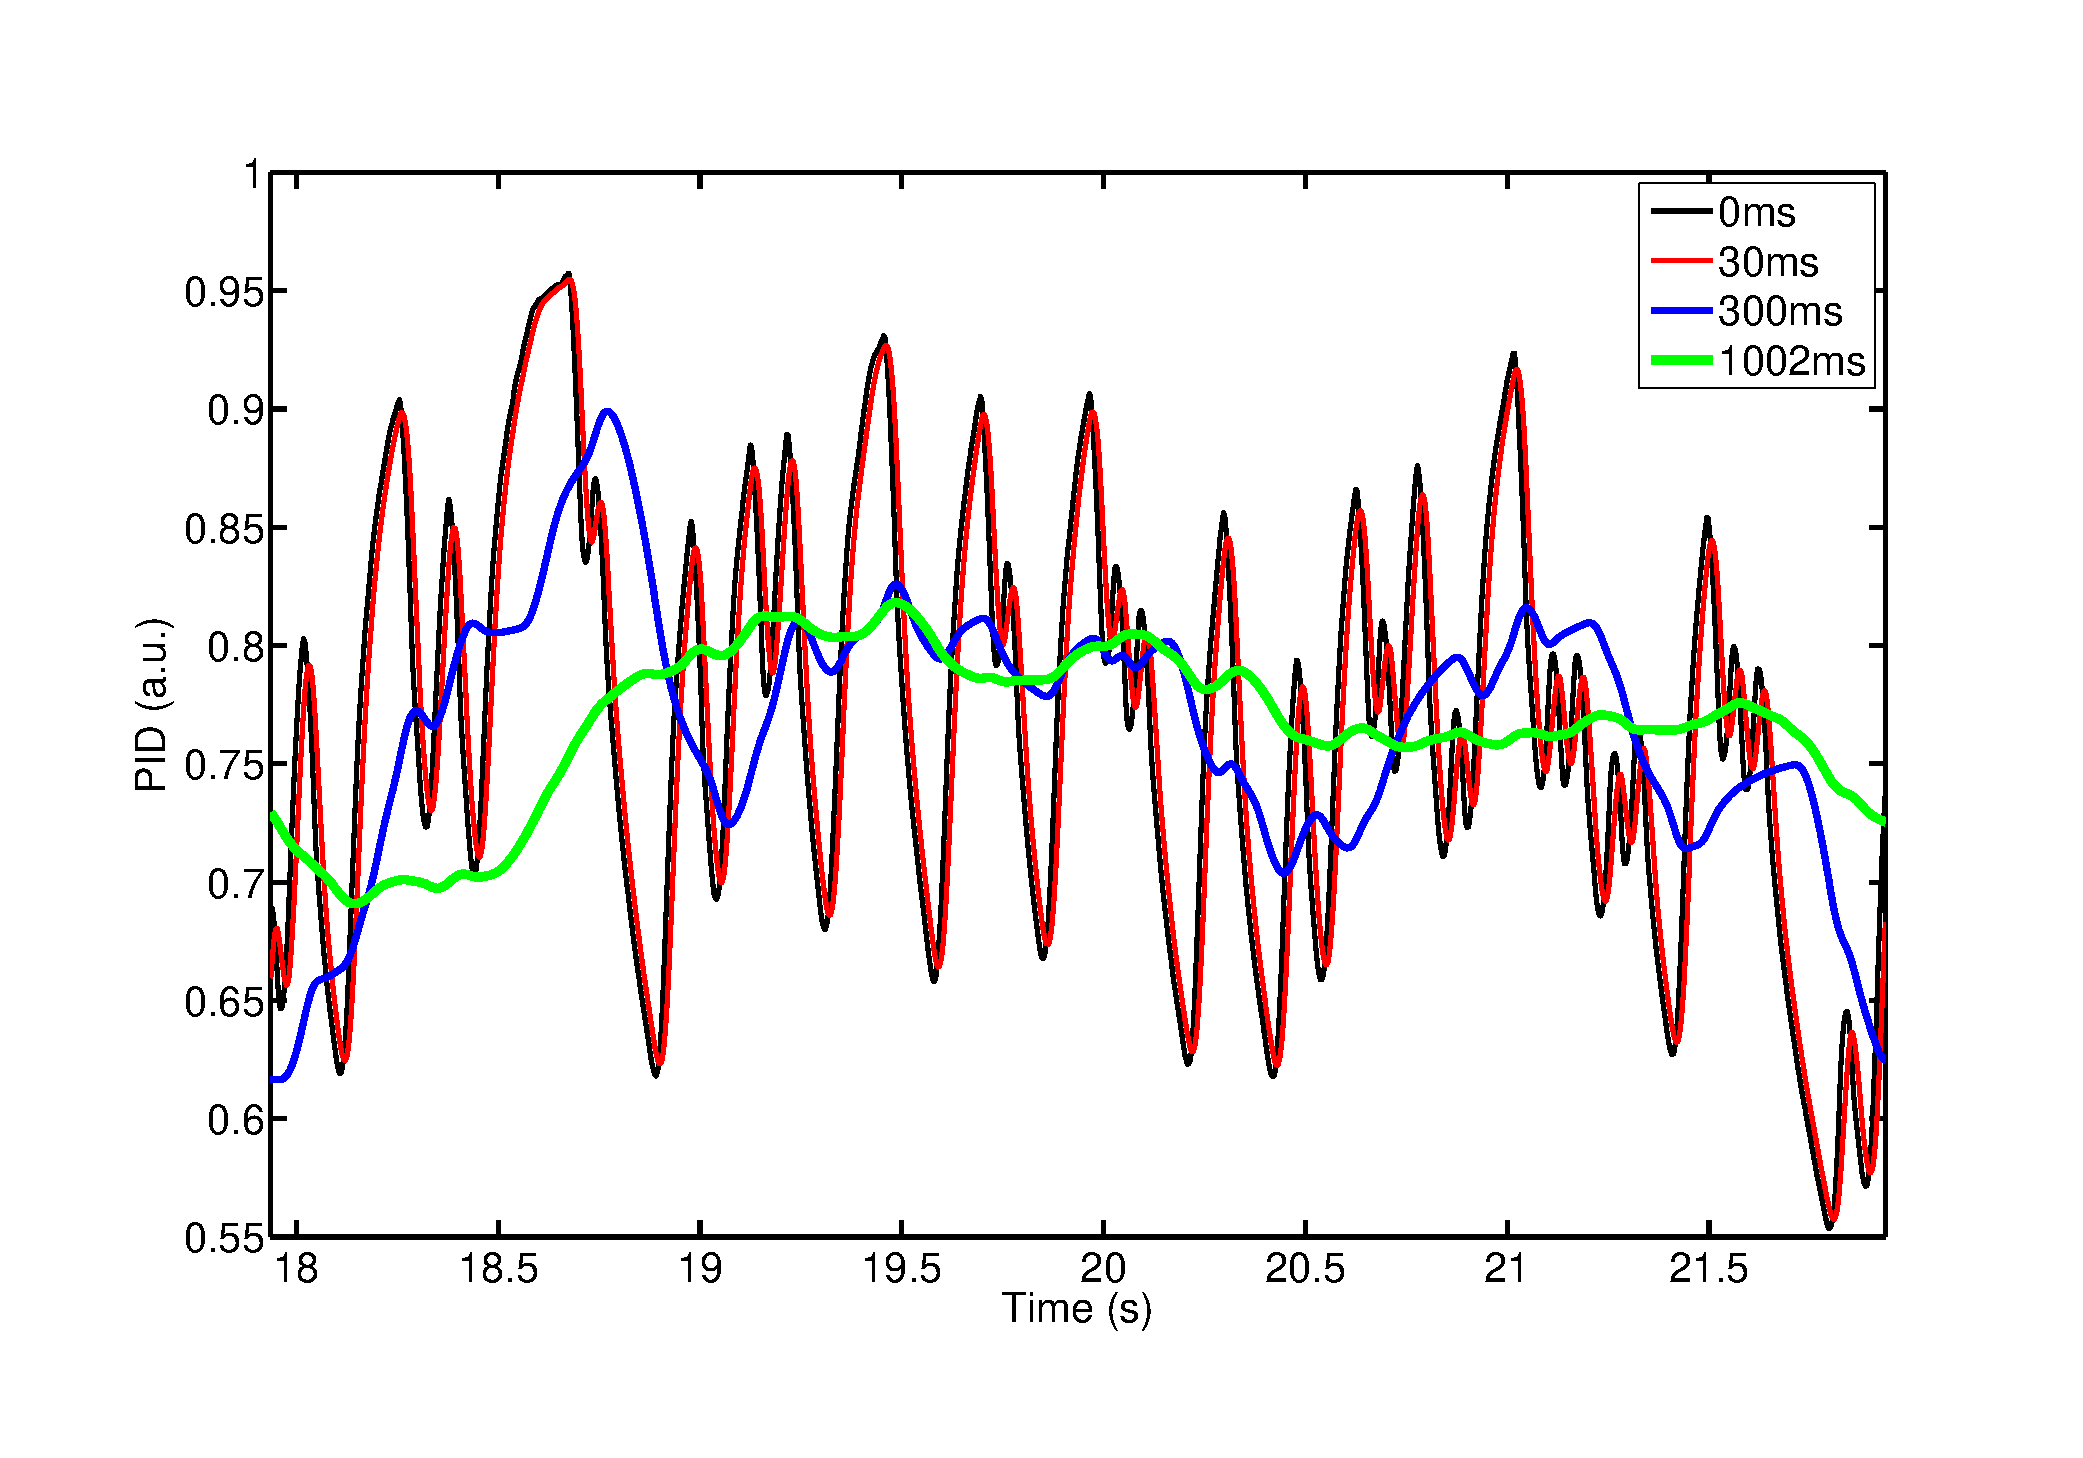
\includegraphics [width=\textwidth]{Analysis_January_07.pdf}
\begin{par}
Now, we separate neuron responses and linear prediction at times when the mean average stimulus is in the lowest 10\% or the highest 10\%. These points are marked either green (lowest 10\%) or red (or highest 10\%) in the figures below, while all the data is plotted in grey. Lines are fit to each of these clouds of points, and the slopes (representing the instantaneous gain) is calculated from these lines. The \textit{y} axis is the actual firing rate, while the \textit{x} axis is the predicted firing rate. In this analysis the prediction from the PID is used.
\end{par} \vspace{1em}

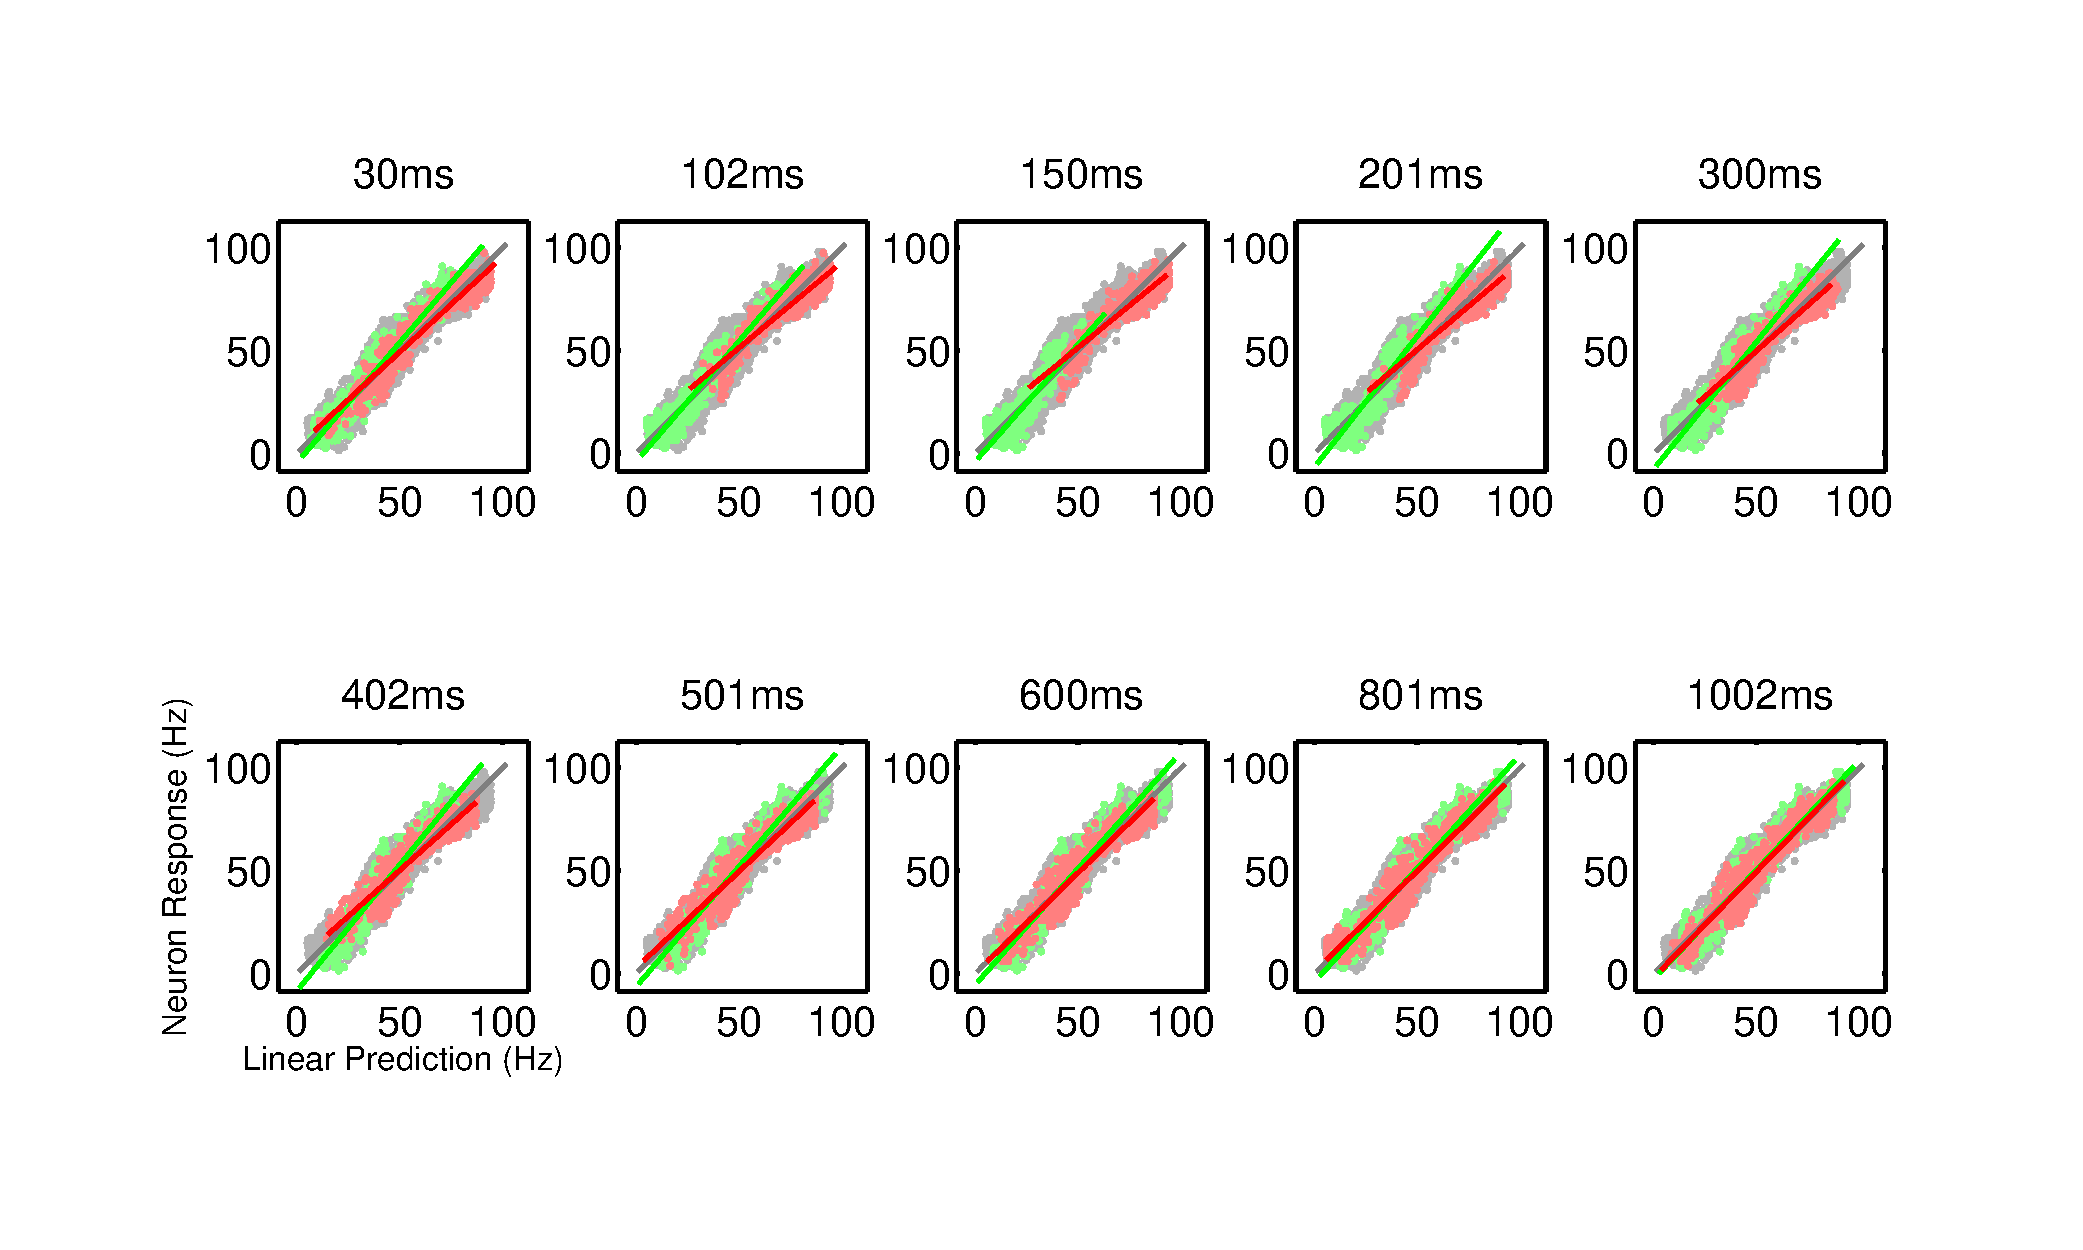
\includegraphics [width=\textwidth]{Analysis_January_08.pdf}
\begin{par}
The following plot shows how the slope of the lines of best fit, or the instantaneous gains, varies with the history length. The plot on the right shows the goodness of fit for each fit, indicating the regions where the fit is meaningful.
\end{par} \vspace{1em}

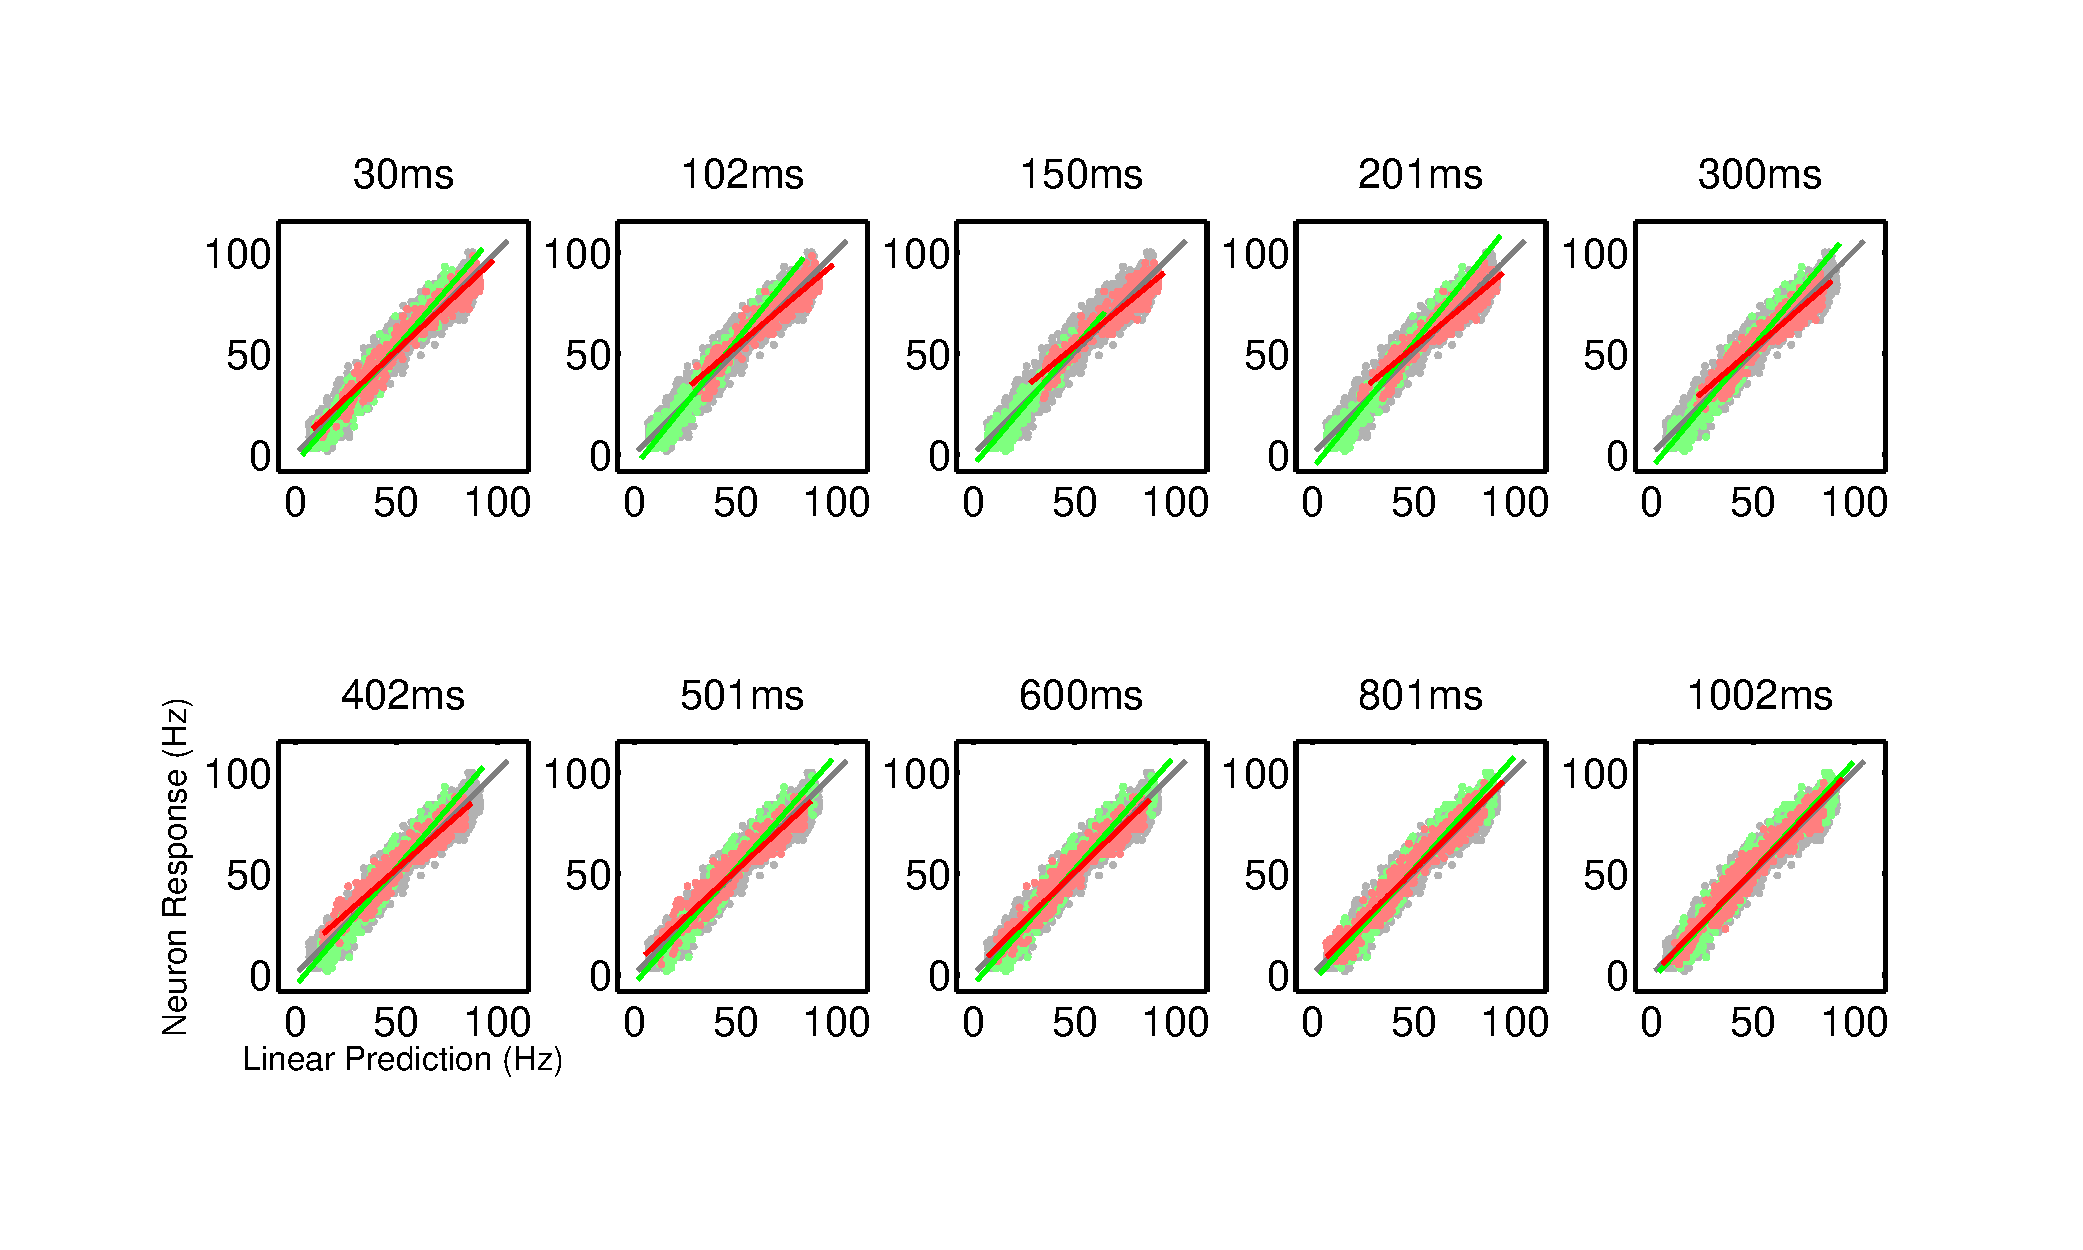
\includegraphics [width=\textwidth]{Analysis_January_09.pdf}


\subsection*{Analysis of Linear Prediction - Filter Variation}

\begin{par}
We have segmented the entire data set based on when the stimulus, averaged in some way over the past, into high and low. The following plots show how the filter shape for low, high and middle 10\% of the stimuli changes with the history window size. In these plots, only 10\% of the data, either the lowest 10\% (green), the highest 10\% (red) of the middle 10\% (black), based on the window smoothing is used to compute each of the filters.
\end{par} \vspace{1em}

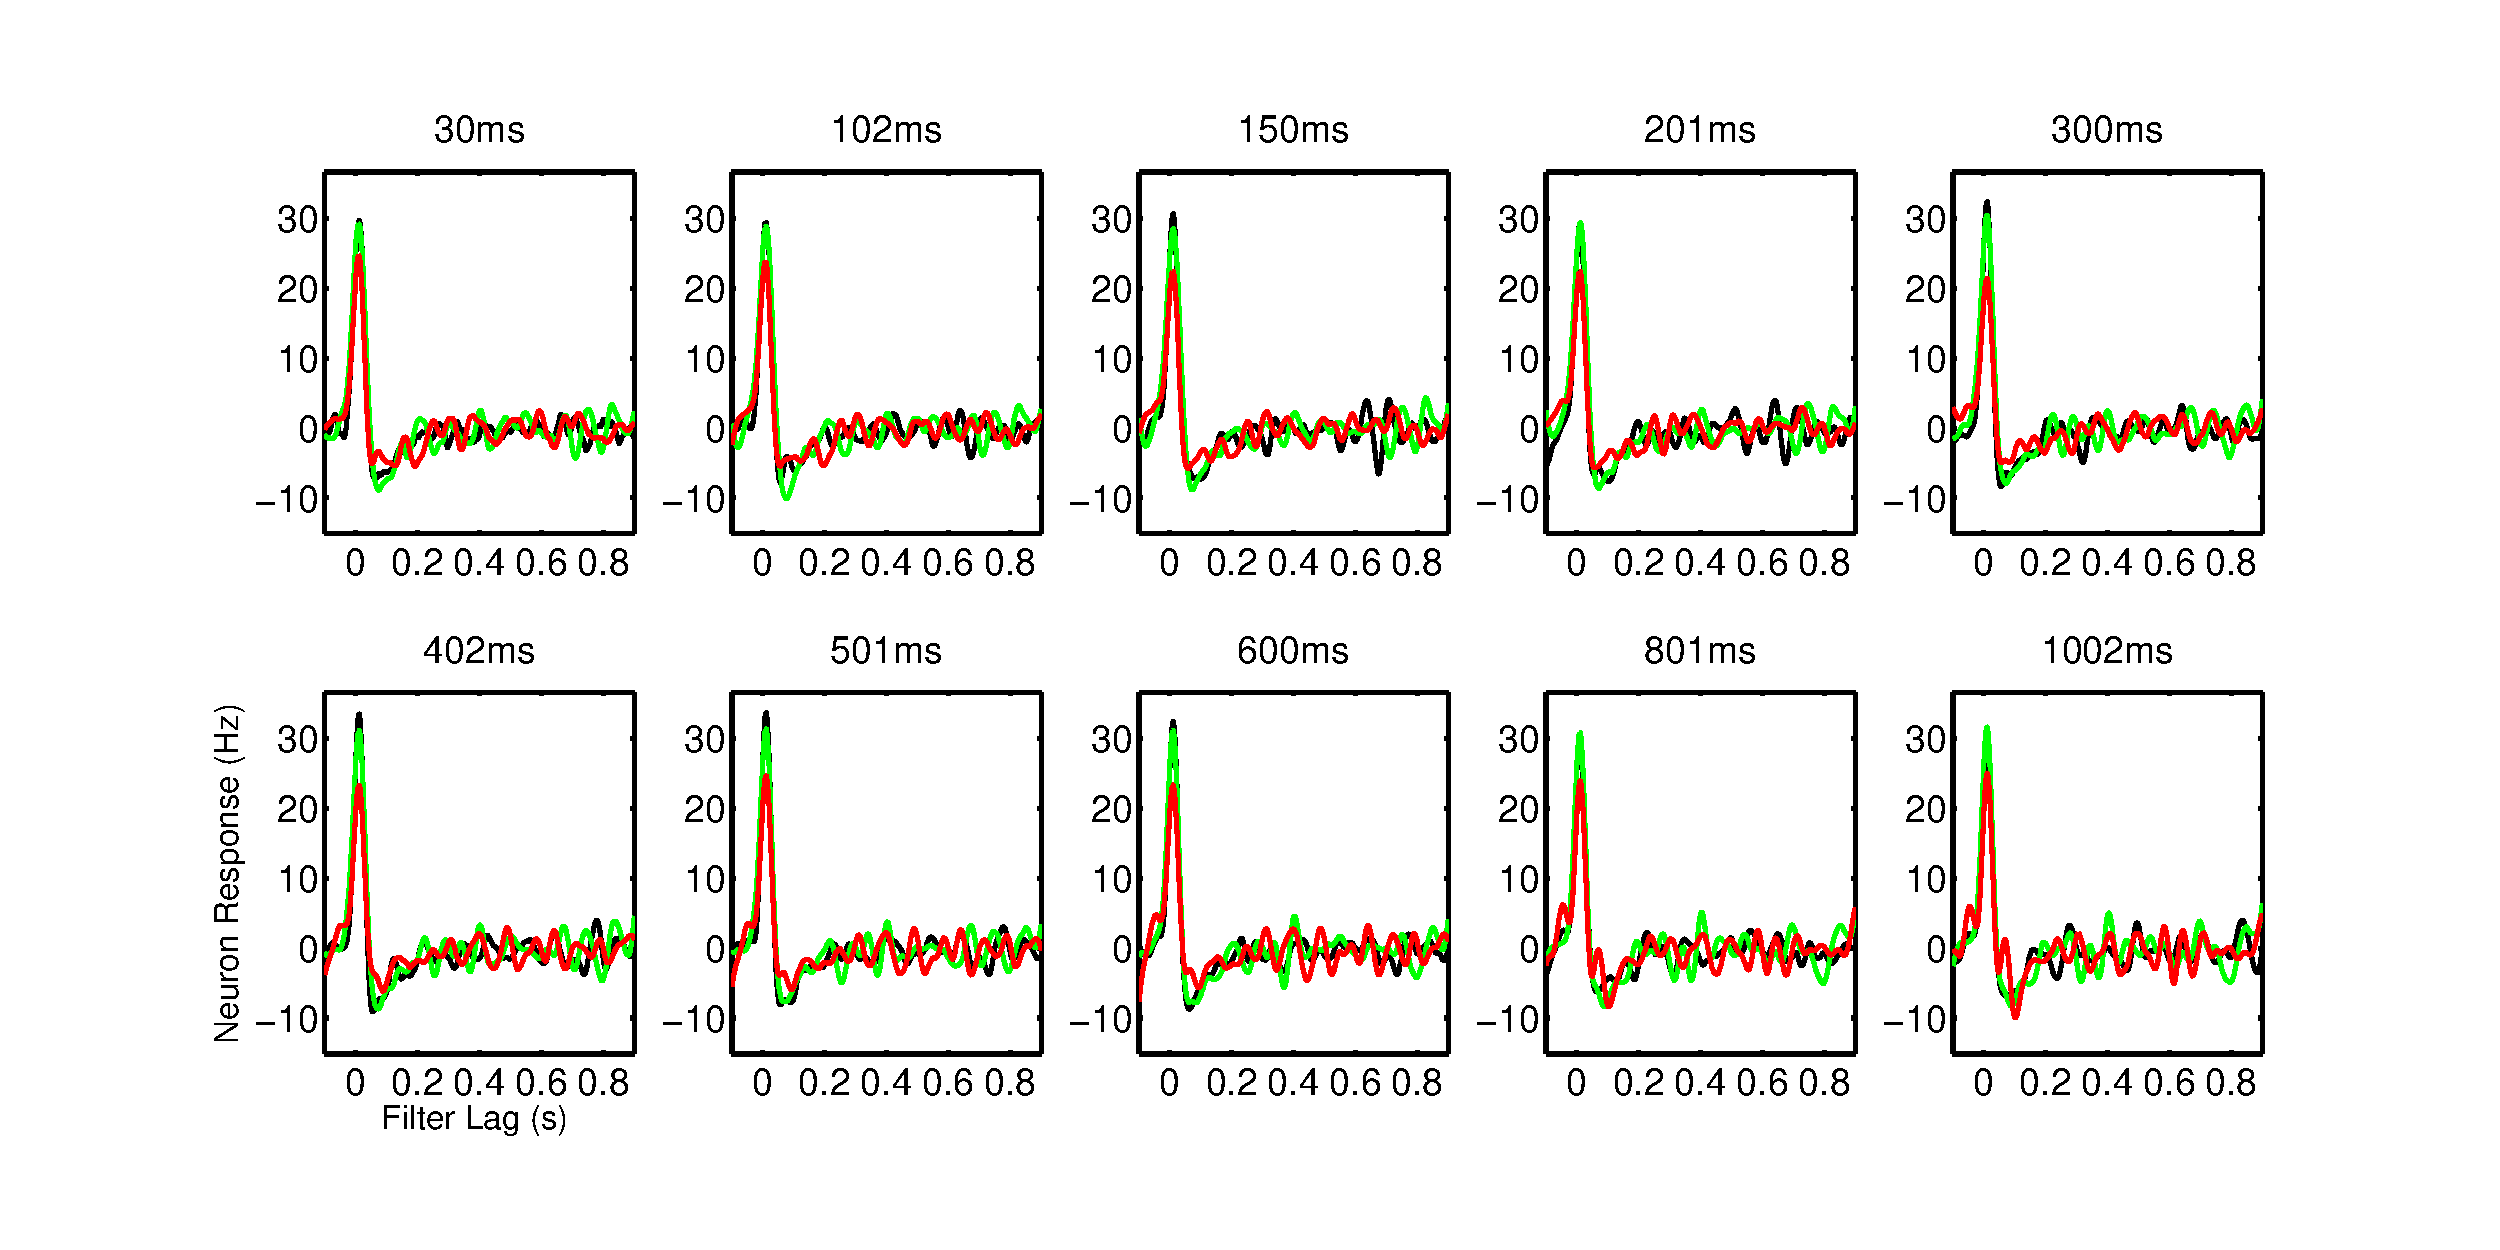
\includegraphics [width=\textwidth]{Analysis_January_10.pdf}
\begin{par}
We can also plot the height of the filter \textit{vs.} the history window size:
\end{par} \vspace{1em}

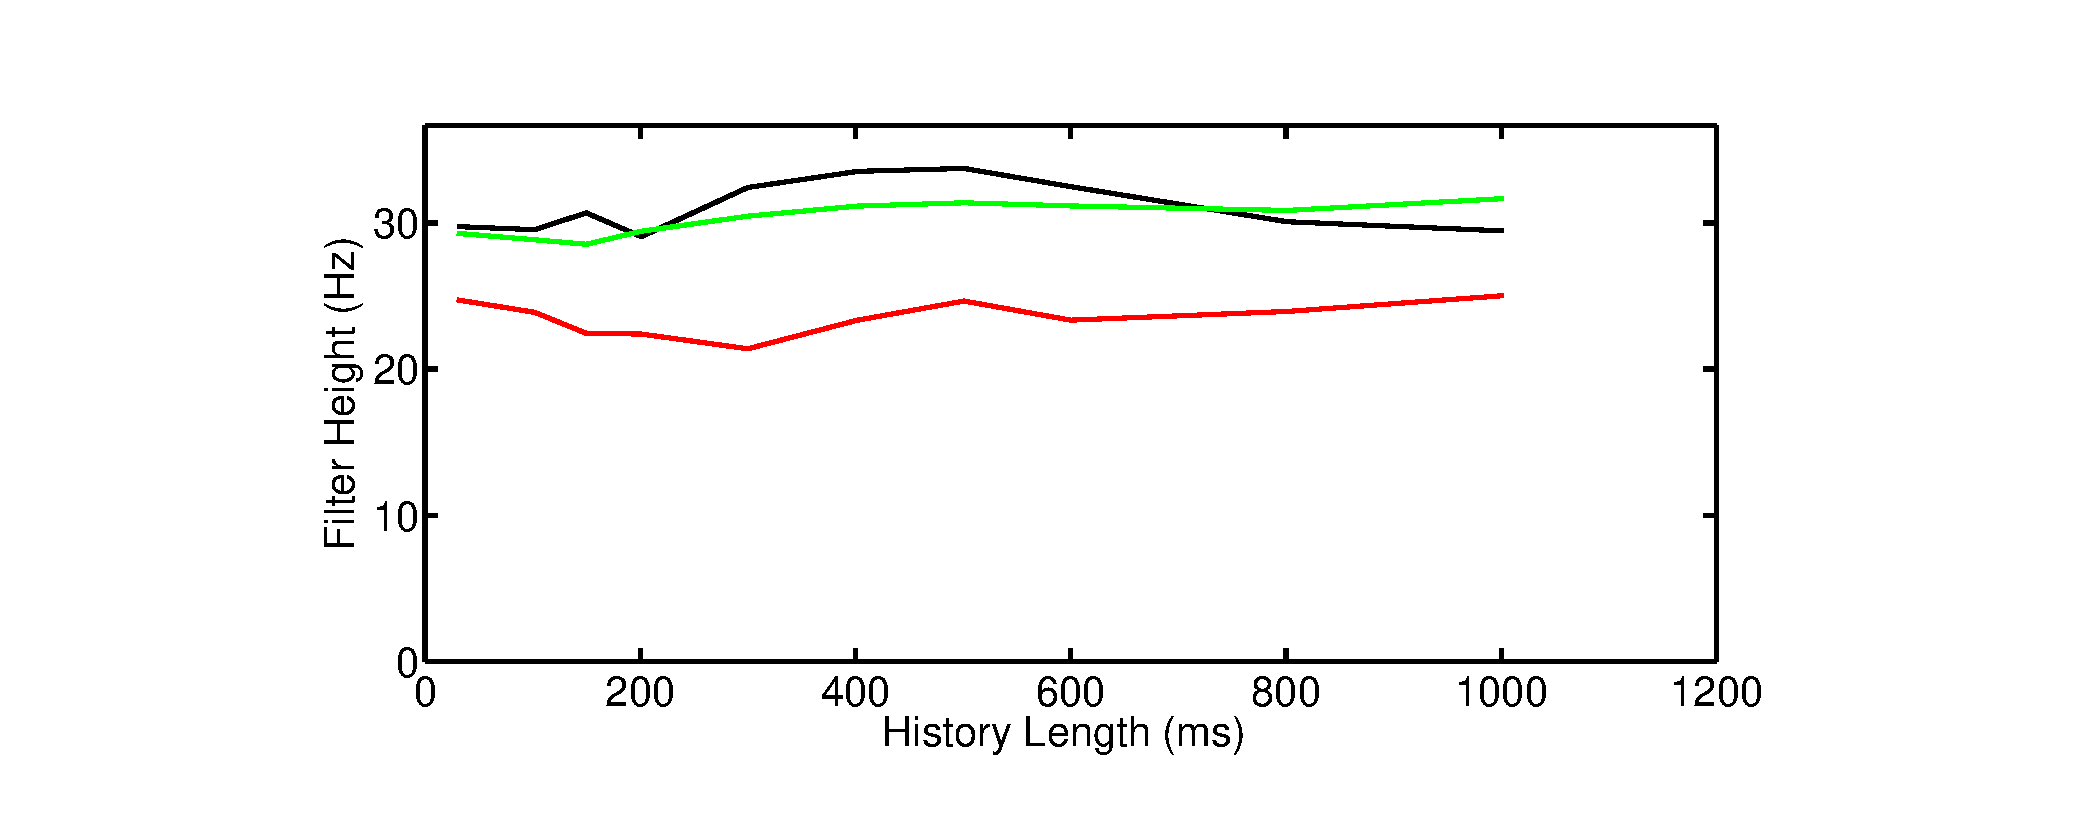
\includegraphics [width=\textwidth]{Analysis_January_11.pdf}
\begin{par}
We also expect the low stimulus (high gain) filter to be slower than the high stimulus (low gain) filter. Is this so in the data? Here, I plot the time of peak of each filter \textit{vs.} the history window size.
\end{par} \vspace{1em}

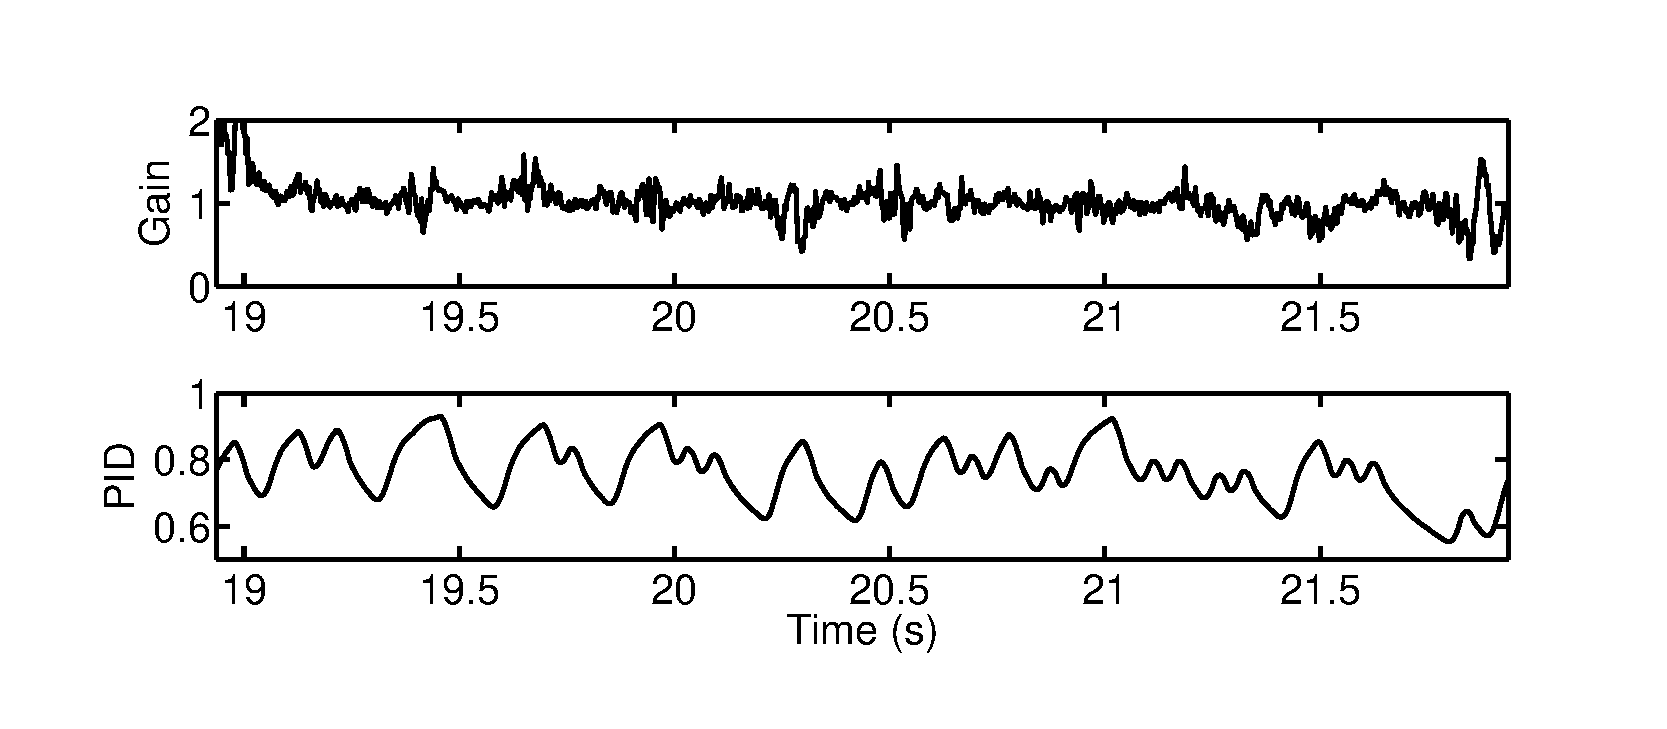
\includegraphics [width=\textwidth]{Analysis_January_12.pdf}


\subsection*{Analysis of Gain: Instantaneous Gain and Fitted Gain}

\begin{par}
There is a mismatch between the linear prediction and the actual firing rate. Moreover, the instantaneous gain seems to be modulated by something that depends on the past history of the stimulus (see analysis in the previous section). We also know that we cannot predict with a simple linear filter any linear errors that the filter makes. However, there is the possibility of fitting a linear filter to the gain, which is a non-linear function of the filter output. But how do we compute this gain? Here, in the figure below, the instantaneous gain, i.e., the ratio of the actual firing rate to the predicted firing rate, is plotted along with the stimulus.
\end{par} \vspace{1em}

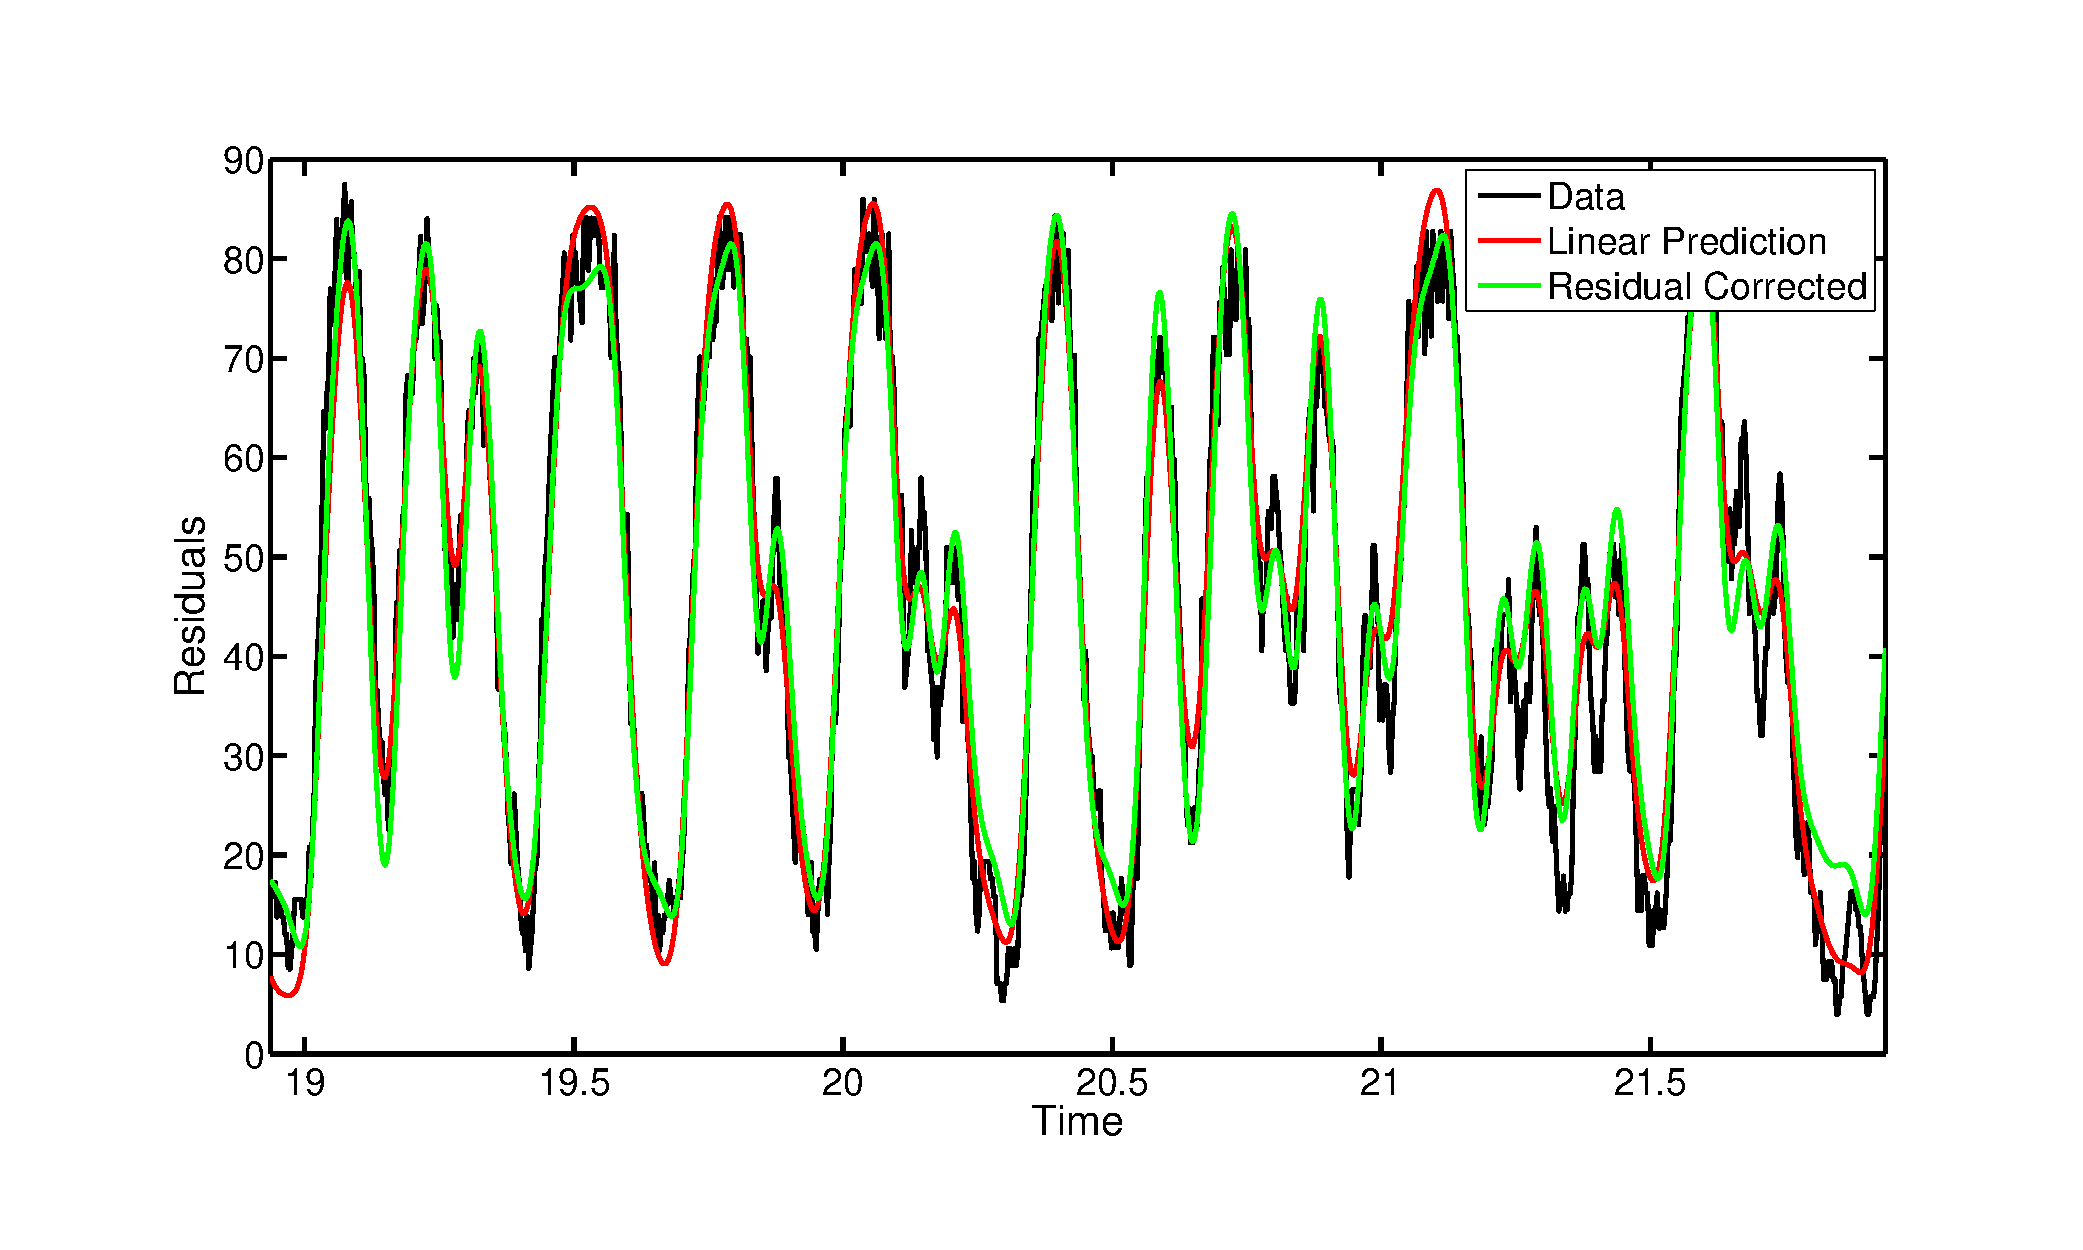
\includegraphics [width=\textwidth]{Analysis_January_13.pdf}
\begin{par}
We can also calculate the moving gain by fitting lines to the data and the prediction collected in bins of size \textit{w}. The following plots show the gain computed in this way for a few different \textit{w}. We want to do this because the raw instantaneous gain is very noisy, and predicting it from PID is hard.
\end{par} \vspace{1em}

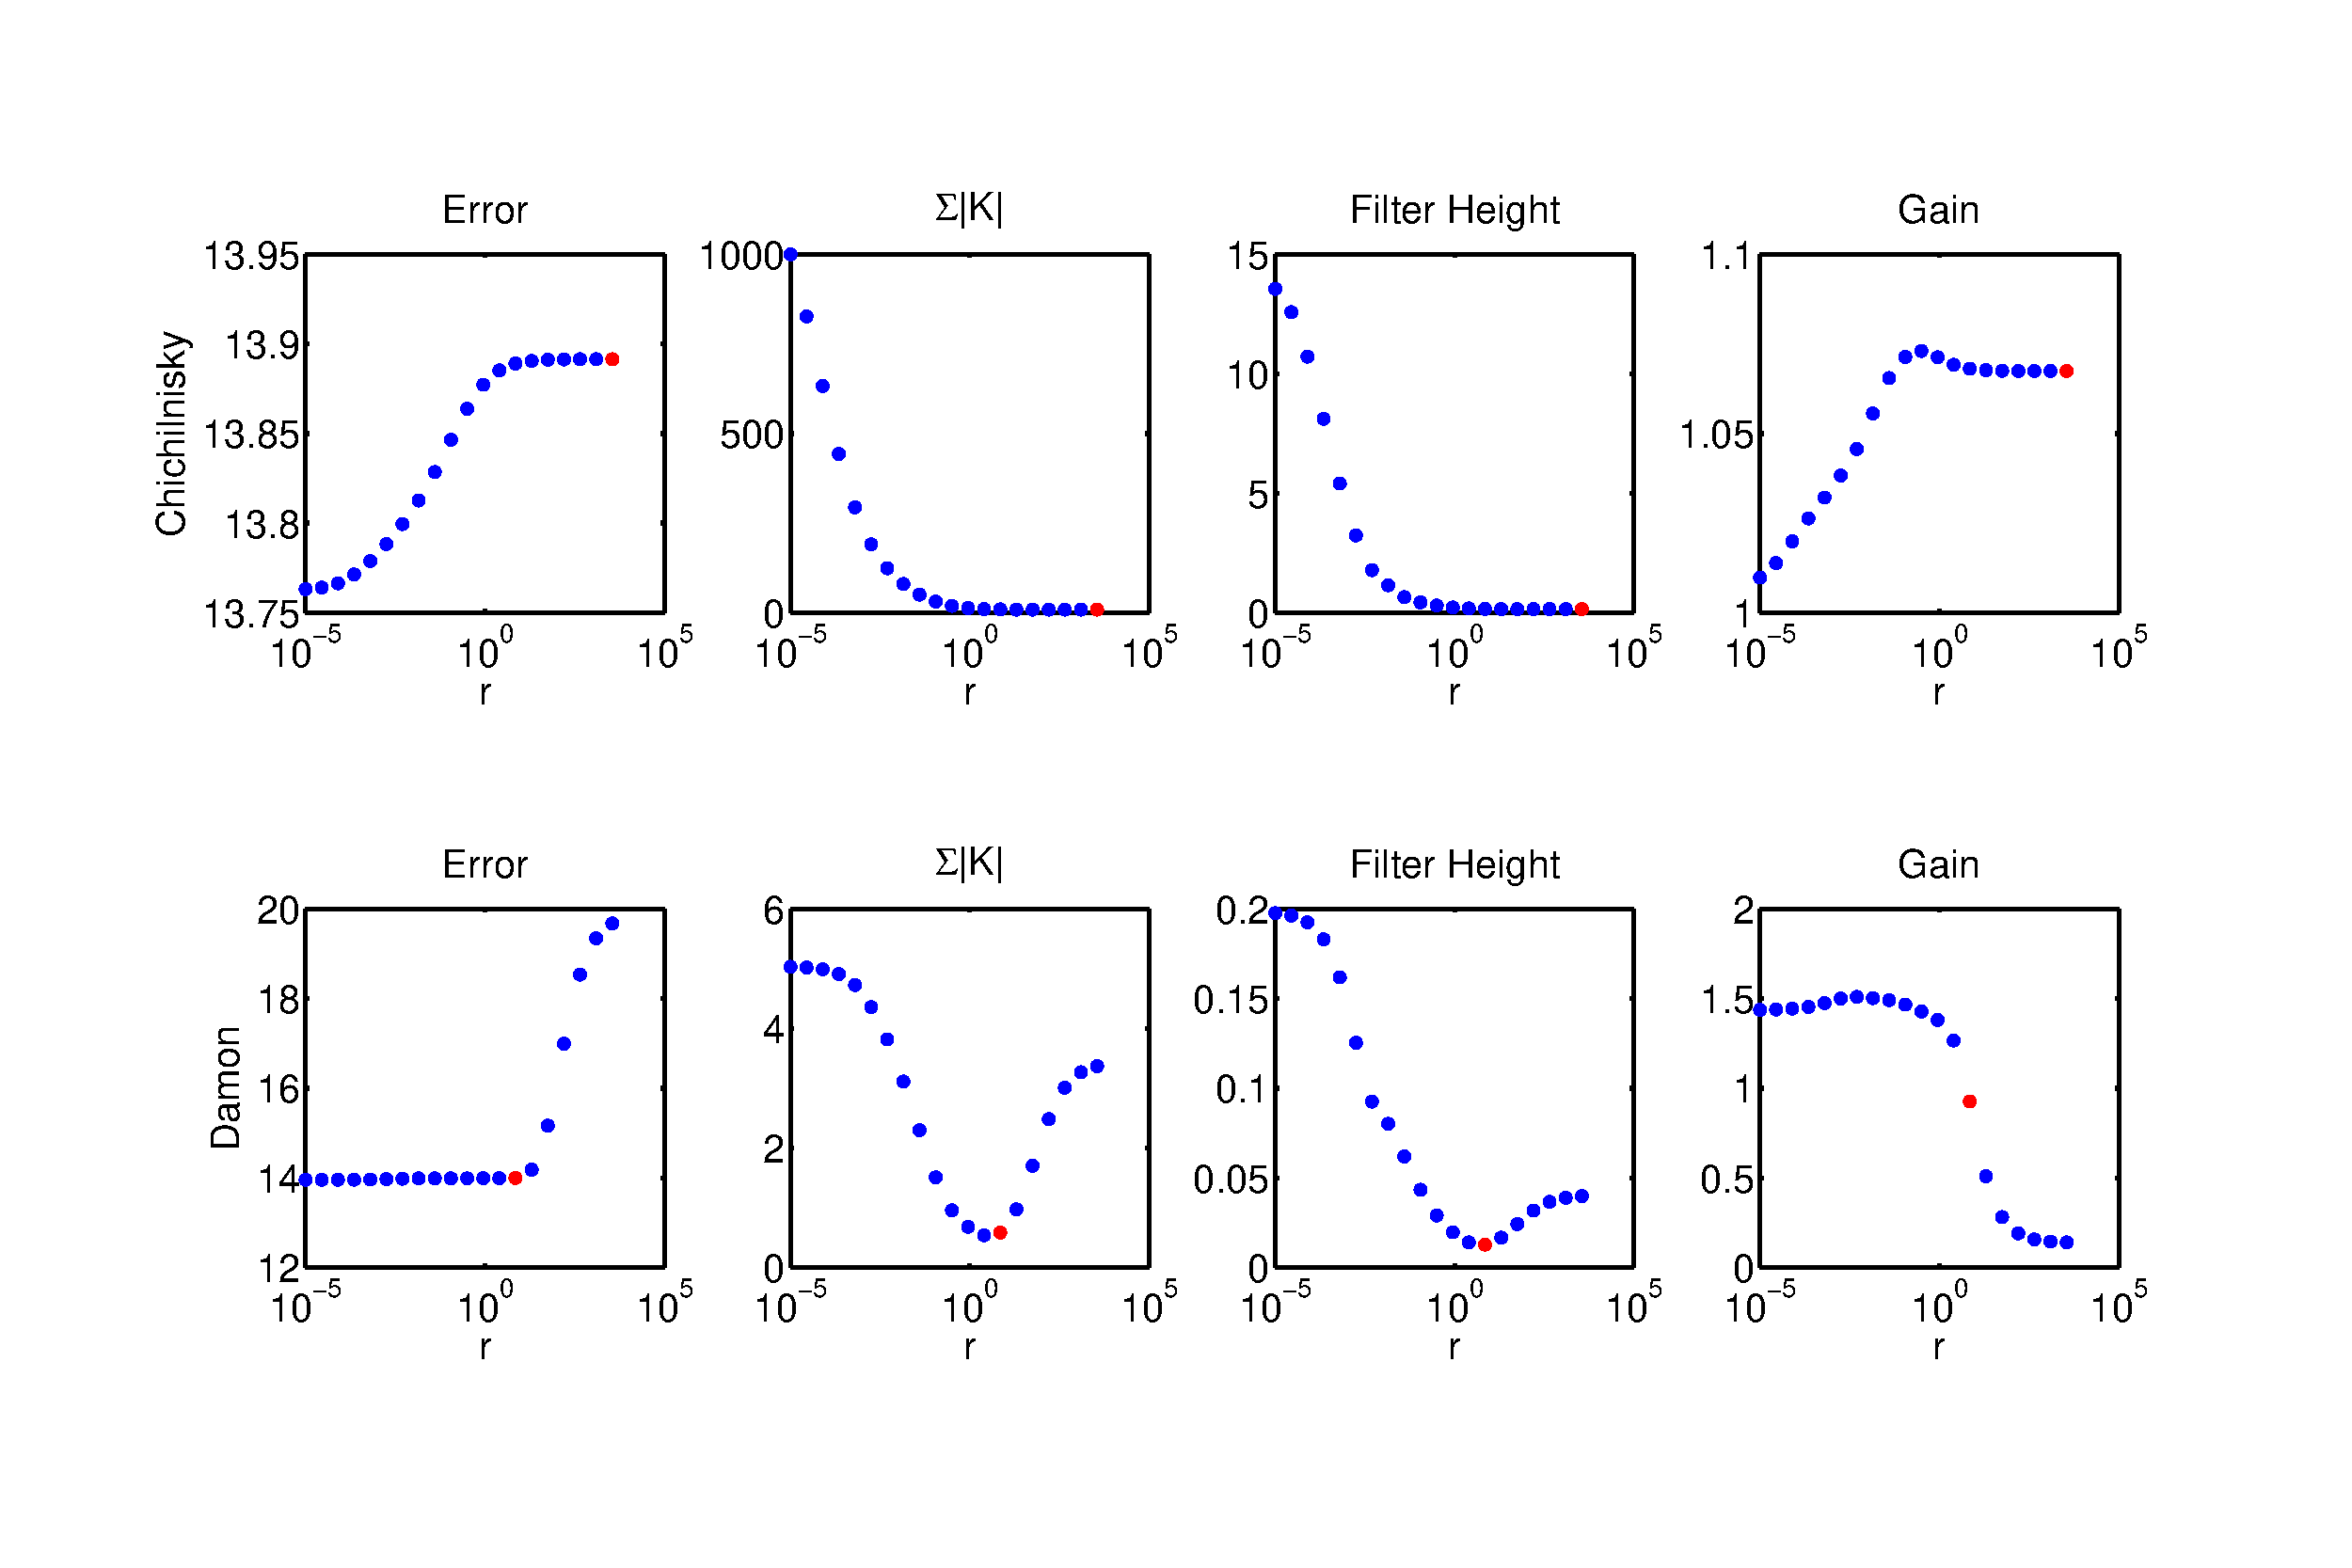
\includegraphics [width=\textwidth]{Analysis_January_14.pdf}
\begin{par}
Of these different gain vectors, which fixes the prediction the best? The following plot shows the r-square values of corrected linear prediction, corrected by the gain computed in different ways (lines fit to windows of different lengths). On the y-axis is the r-square, and the x-axis is the window over which the lines are fit.  The first point has a r-square of 1, indicating a perfect fit (this is by definition, since the first point is the instantaneous gain). Note that none of the other points exceed the line, which indicates the r-square of the simple linear prediction.
\end{par} \vspace{1em}

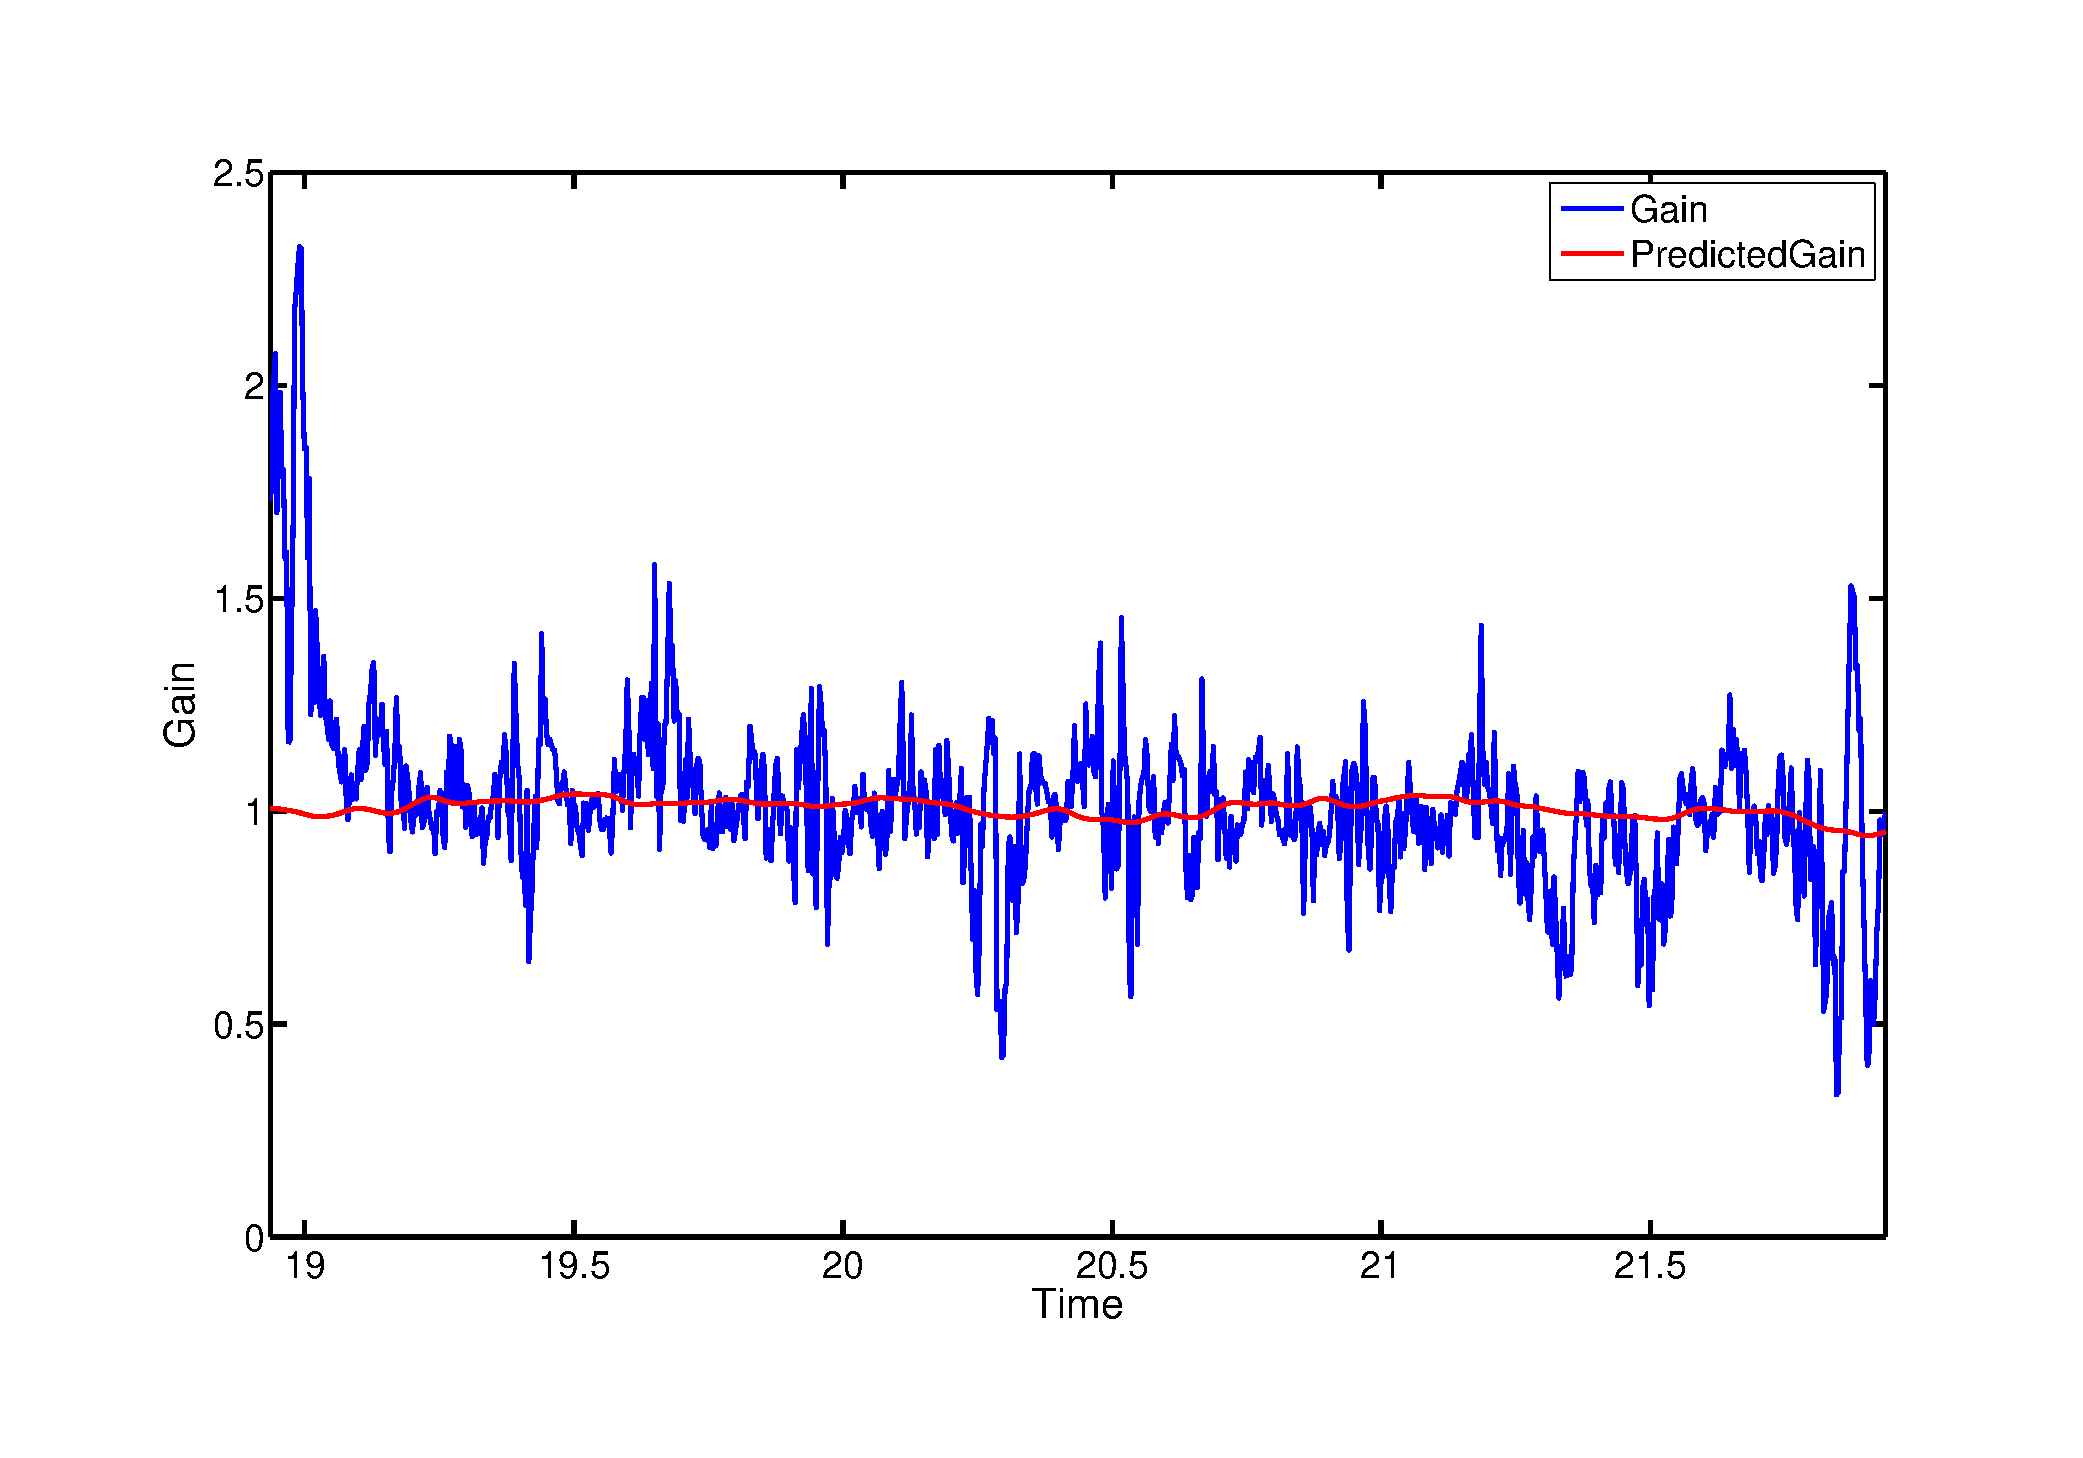
\includegraphics [width=\textwidth]{Analysis_January_15.pdf}
\begin{par}
We conclude that this method of finding the gain is not helpful in improving the prediction.
\end{par} \vspace{1em}


\subsection*{Analysis of Gain: Smoothed gain.}

\begin{par}
Instead of calculating the instantaneous point-by-point gain, we can also smooth the instantaneous gain over some small window size \textit{w}. The following plot shows the effect of smoothing for a few window sizes \textit{w}.
\end{par} \vspace{1em}

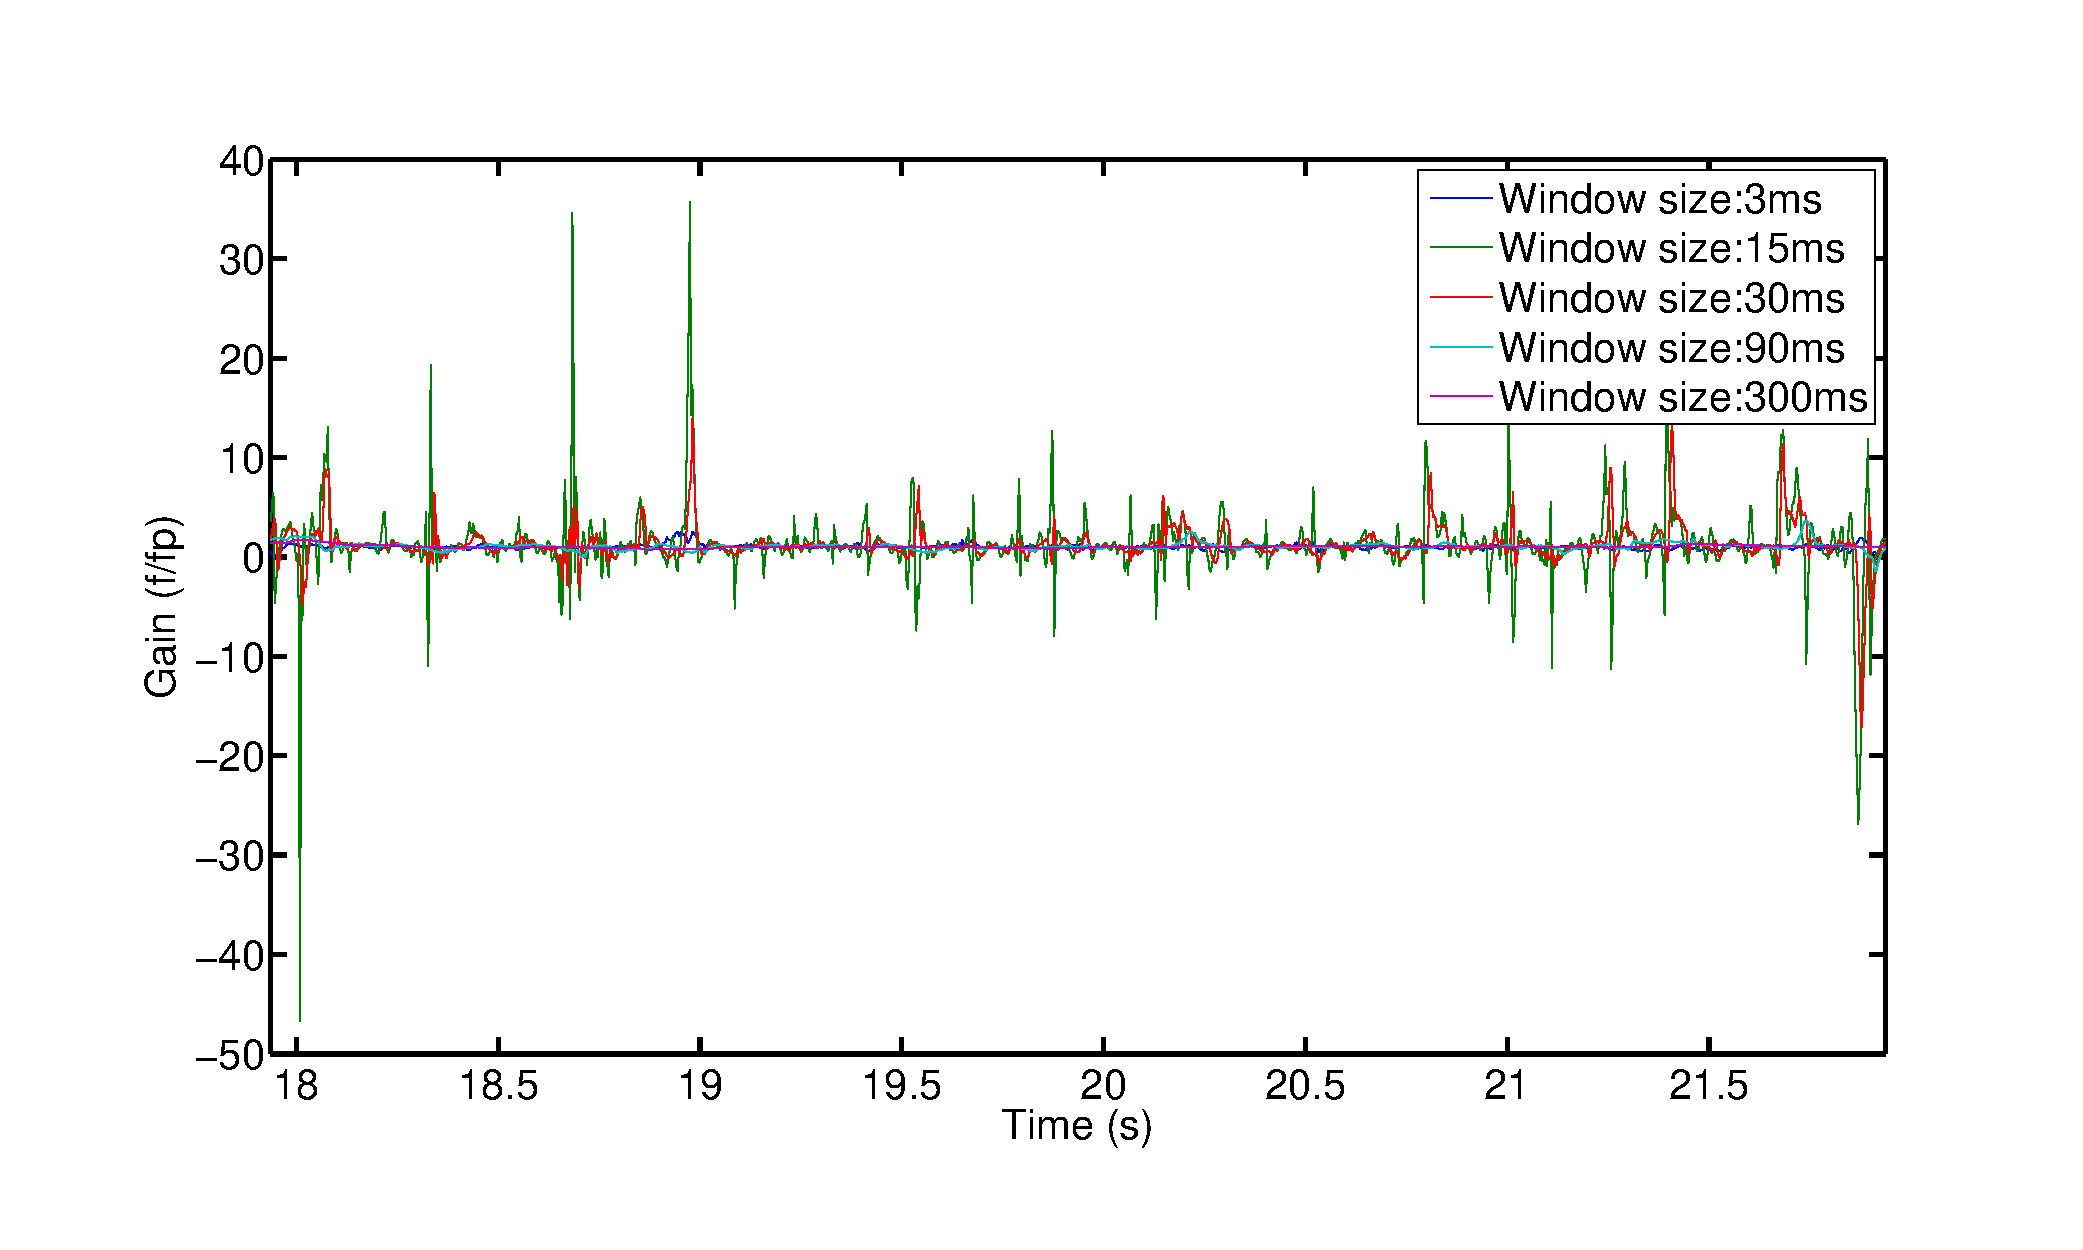
\includegraphics [width=\textwidth]{Analysis_January_16.pdf}
\begin{par}
How does smoothing the gain affect our ability to correct the linear prediction? The following plot shows how the r-square of the corrected linear prediction varies with smoothing the gain. Also shown is the line which indicates the linear prediction of the uncorrected simple linear prediction.
\end{par} \vspace{1em}

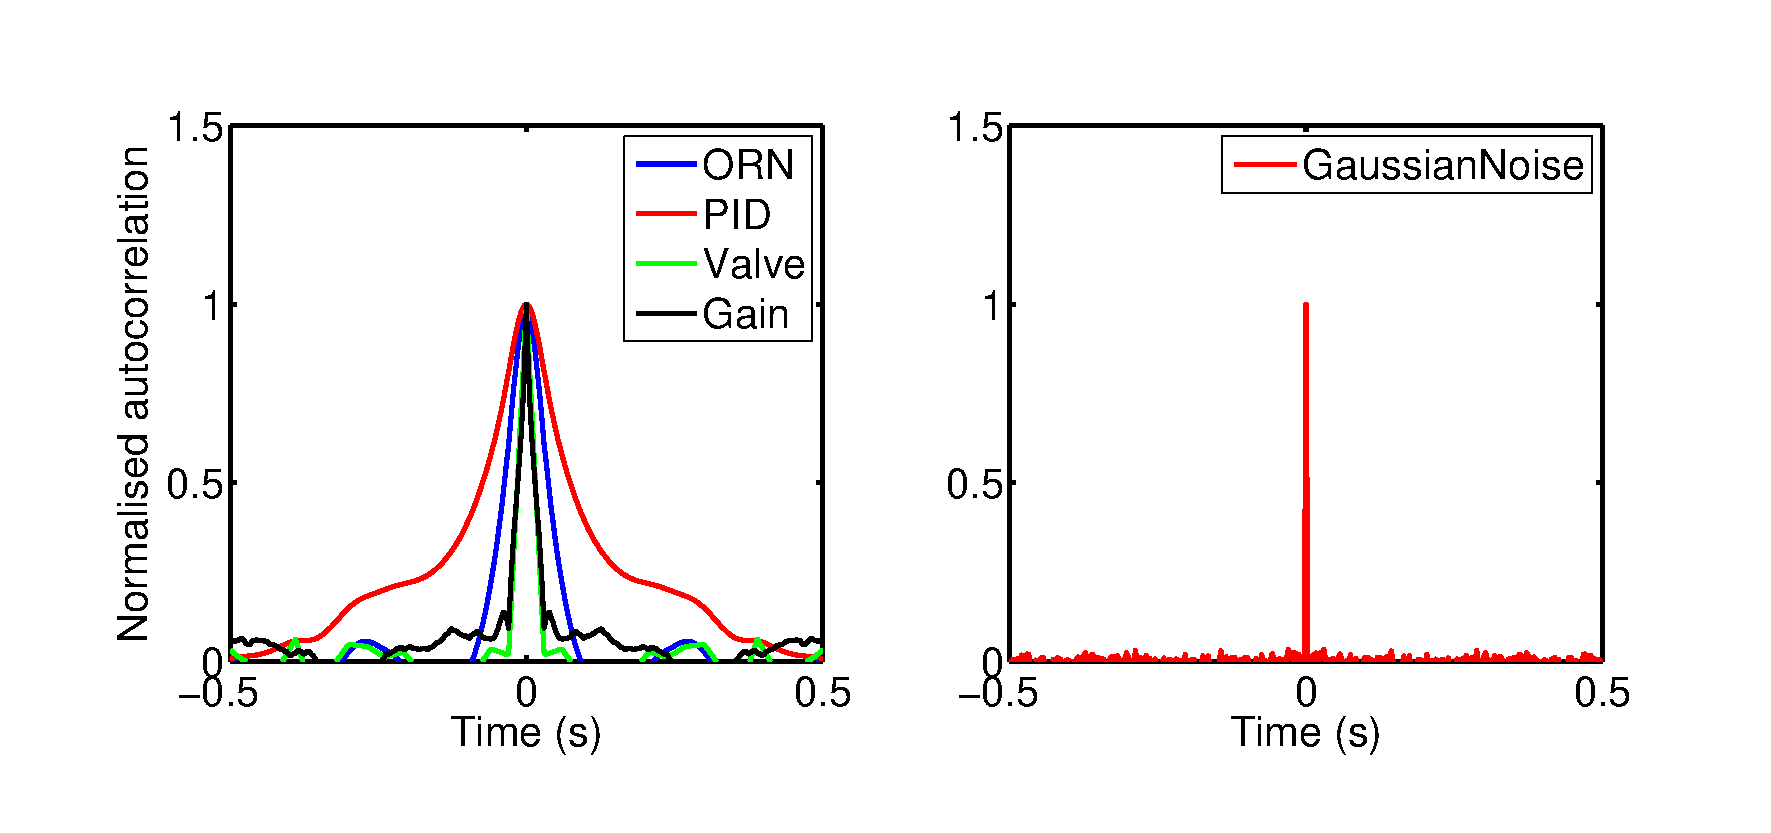
\includegraphics [width=\textwidth]{Analysis_January_17.pdf}
\begin{par}
From this analysis of the gain, it is clear that if we do want to improve the linear prediction, the best way to do it (apart from the instantaneous gain, which would lead to a perfect prediction), is smoothing the gain in some way. In the next section, we will try to estimate the smoothed gain.
\end{par} \vspace{1em}


\subsection*{Gain Analysis - Estimating the gain}

\begin{par}
In the above analysis, we have considered how a boxcar average over the stimulus immediately preceding the current time affects gain. Now, we want to find some optimal way of averaging the past stimulus history to predict the instantaneous gain: by doing so, we can then predict gain, and thus get a better predictor of the actual firing rate.
\end{par} \vspace{1em}
\begin{par}
In effect, we can calculate a new filter, $K_g$ such that
\end{par} \vspace{1em}
\begin{par}
$$ K_g=\hat{C}\setminus(s'*g) $$
\end{par} \vspace{1em}
\begin{par}
where \textit{g} is the smoothed gain and \textit{s} is the stimulus.
\end{par} \vspace{1em}
\begin{par}
For with various smoothing of the instantaneous gain, we find the best filter for each and plot it below:
\end{par} \vspace{1em}

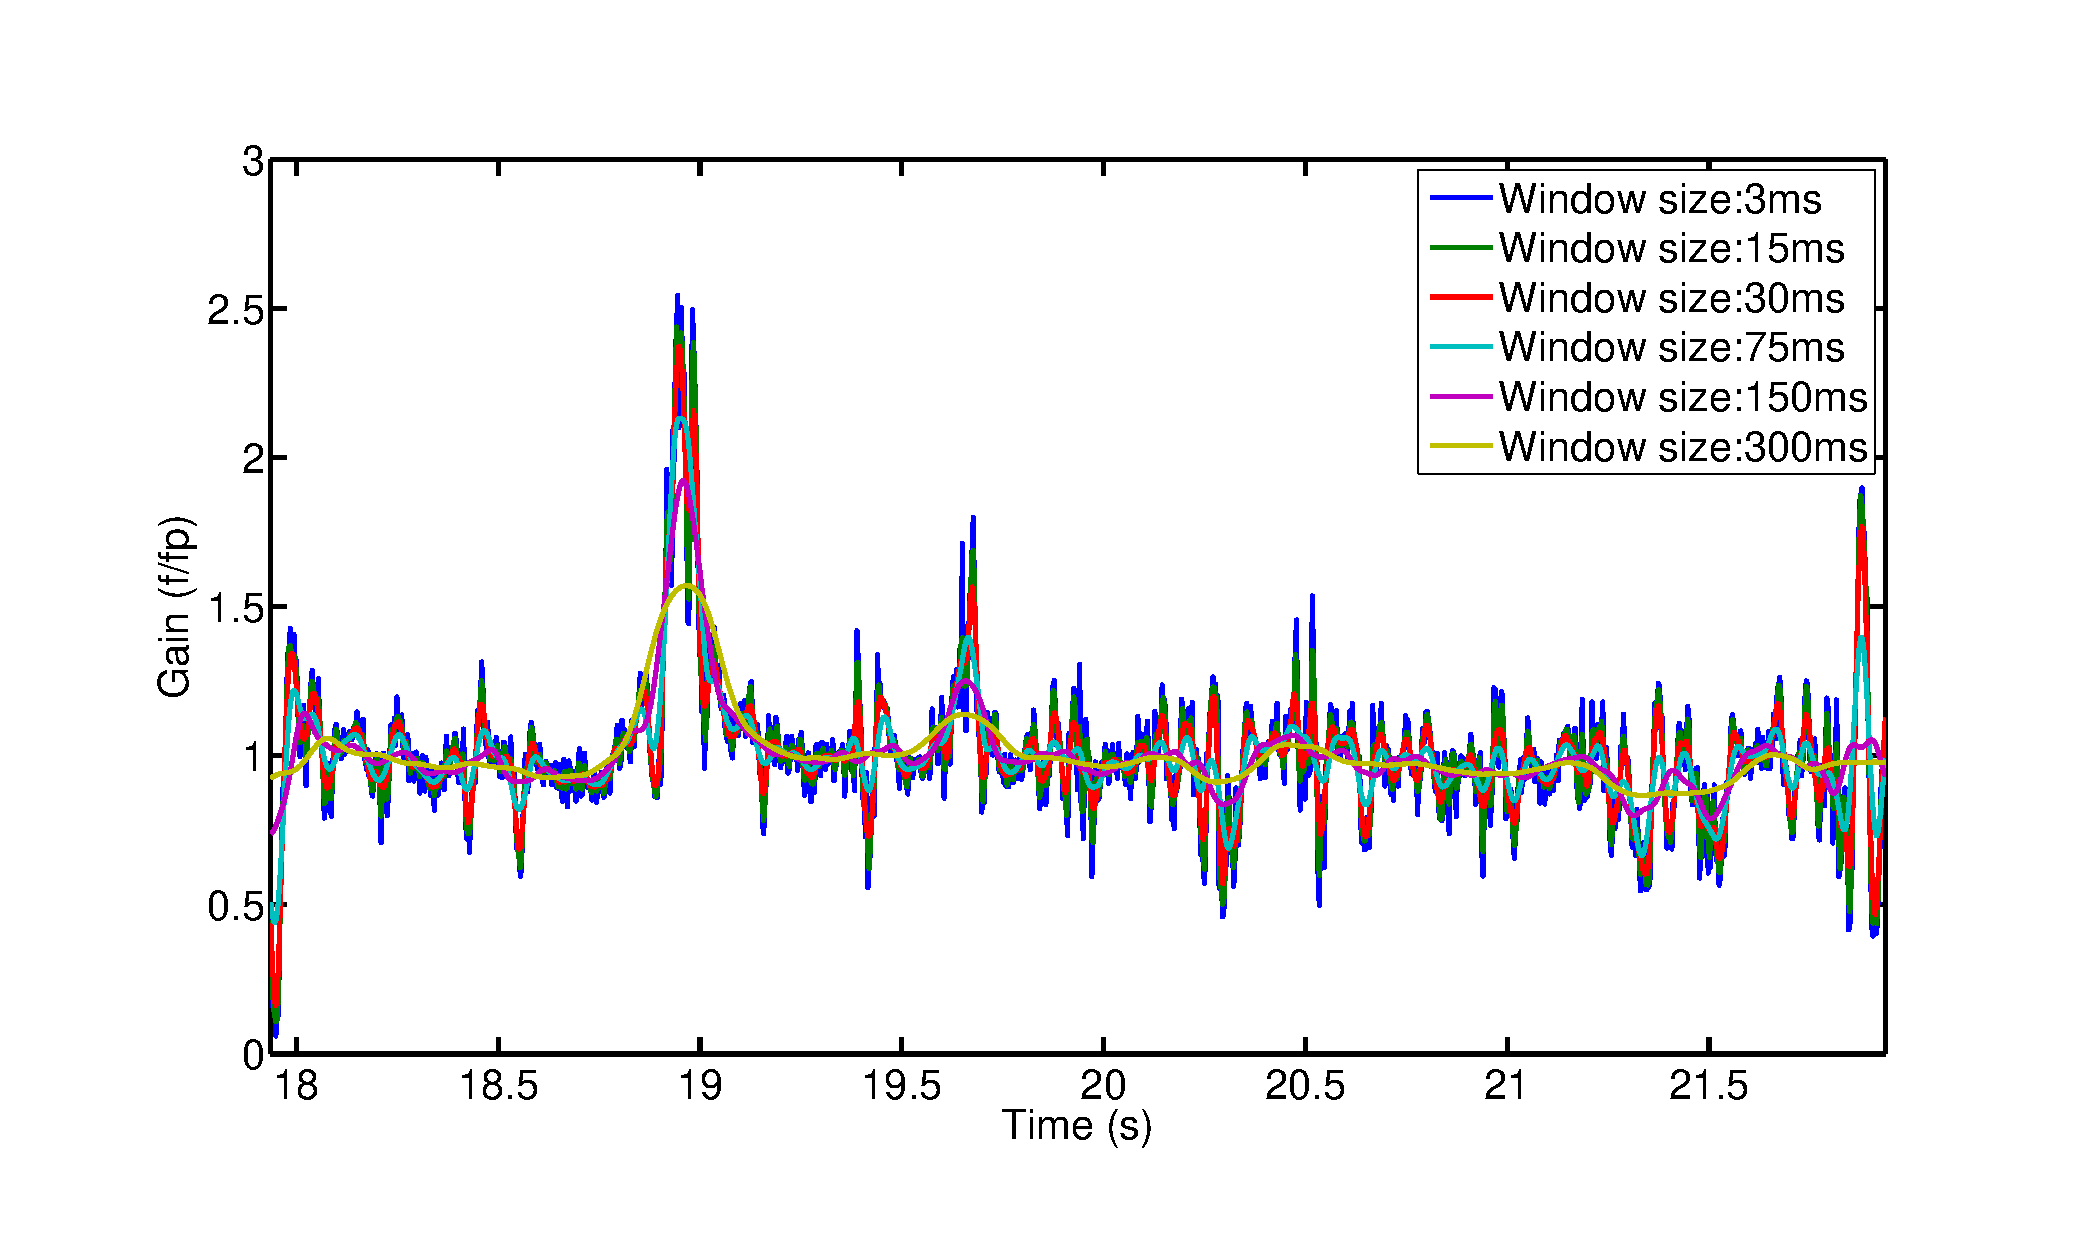
\includegraphics [width=\textwidth]{Analysis_January_18.pdf}
\begin{par}
How well can we predict the smoothed gain vectors using these filters and the stimulus? The following plot shows the r-square between prediction of the smoothed gain and the smoothed gain for various smoothing windows.
\end{par} \vspace{1em}

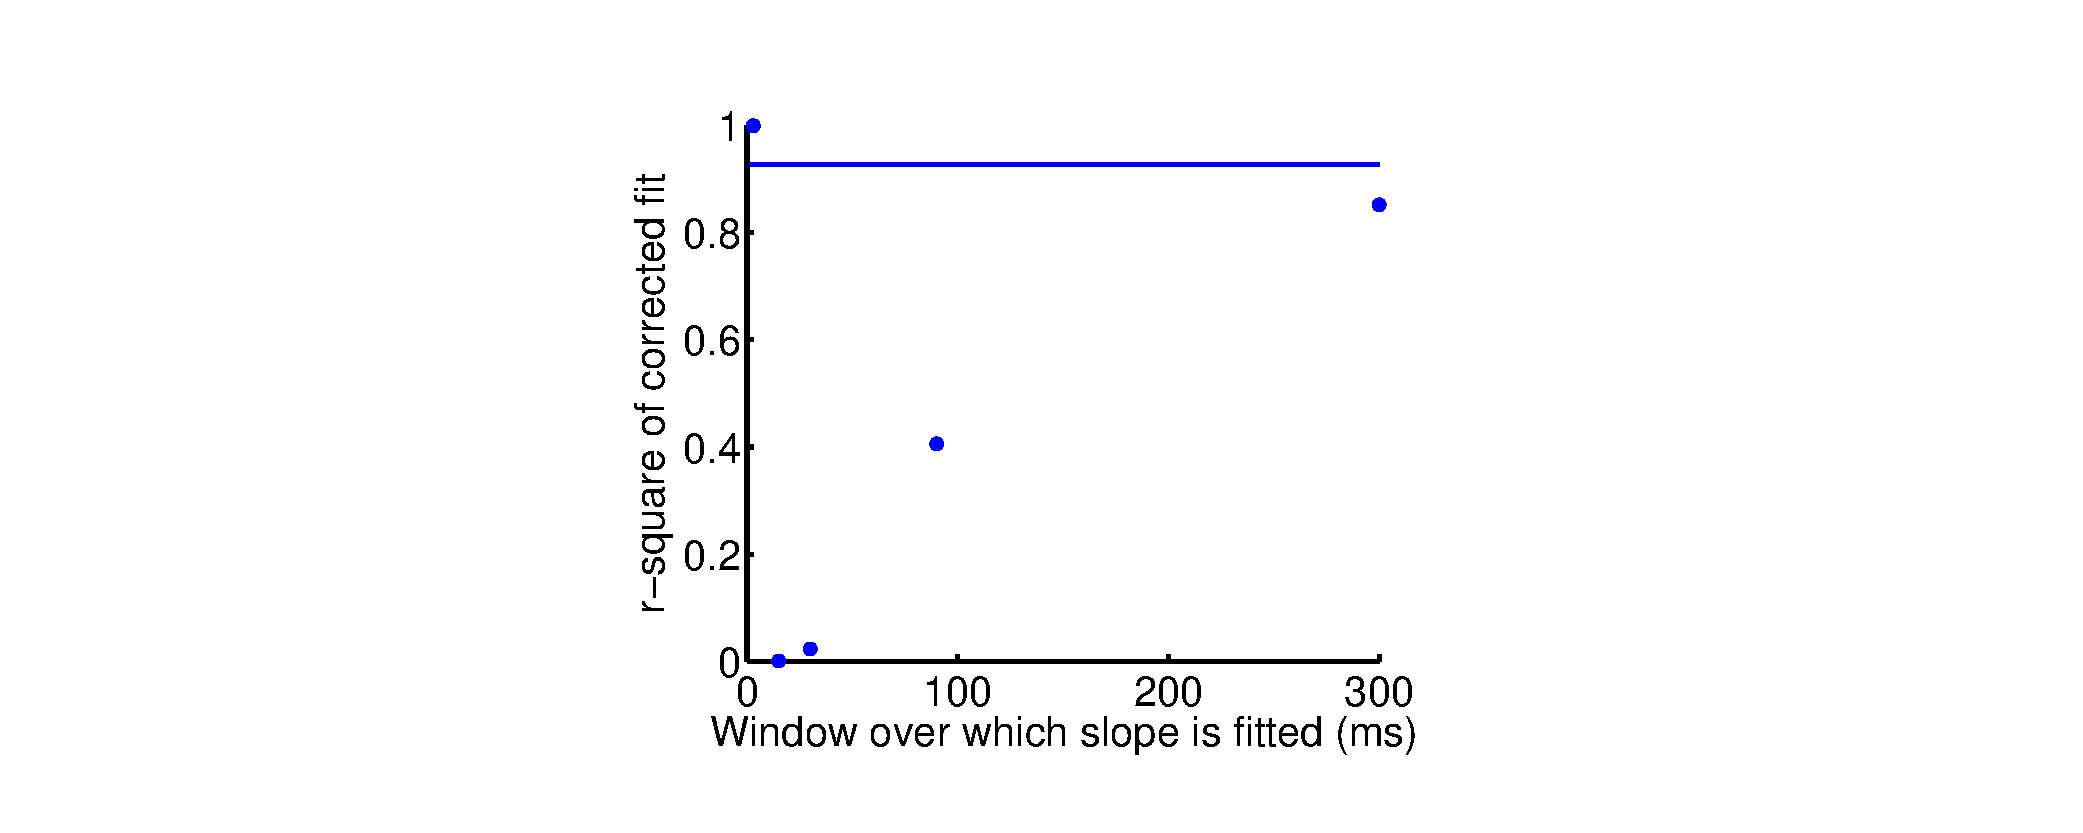
\includegraphics [width=\textwidth]{Analysis_January_19.pdf}
\begin{par}
Well, that sucks. Maybe even this horrible estimation of the gain can improve the linear prediction of the firing rate in some way? Here, I plot the r-square of the gain-corrected linear prediction (corrected by the prediction of the gain), as a function of gain smoothing (in blue). Also plotted is the r-square of the gain-corrected linear prediction, corrected now with actual gain (in black).
\end{par} \vspace{1em}

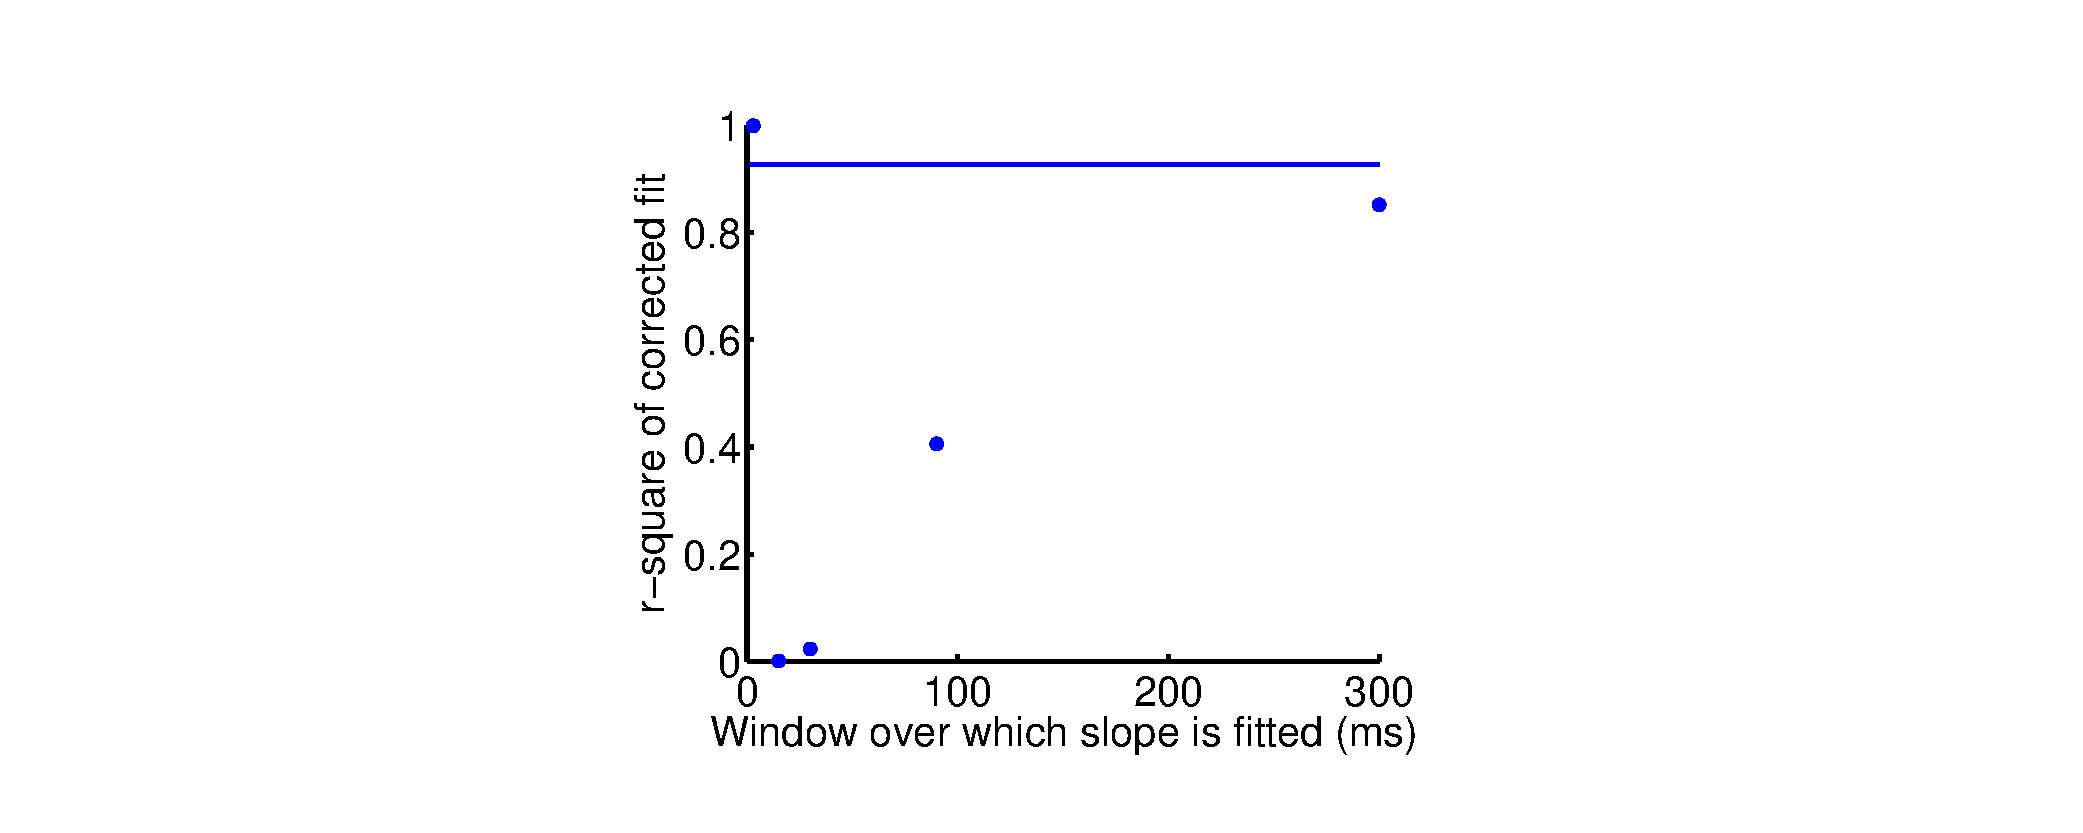
\includegraphics [width=\textwidth]{Analysis_January_20.pdf}


\subsection*{Re-evaluating filter performance after filtering ORN responses}

\begin{par}
The ORN firing rate traces are quite noisy, and it is possible that this is screwing up our estimation of the gain. It is also possible that the linear filter is doing a really good job and can't really be improved, and all the gain residuals are just noise. To check for these possibilities, I will filter the ORN response with a small sliding window, and then recalculate everything.
\end{par} \vspace{1em}

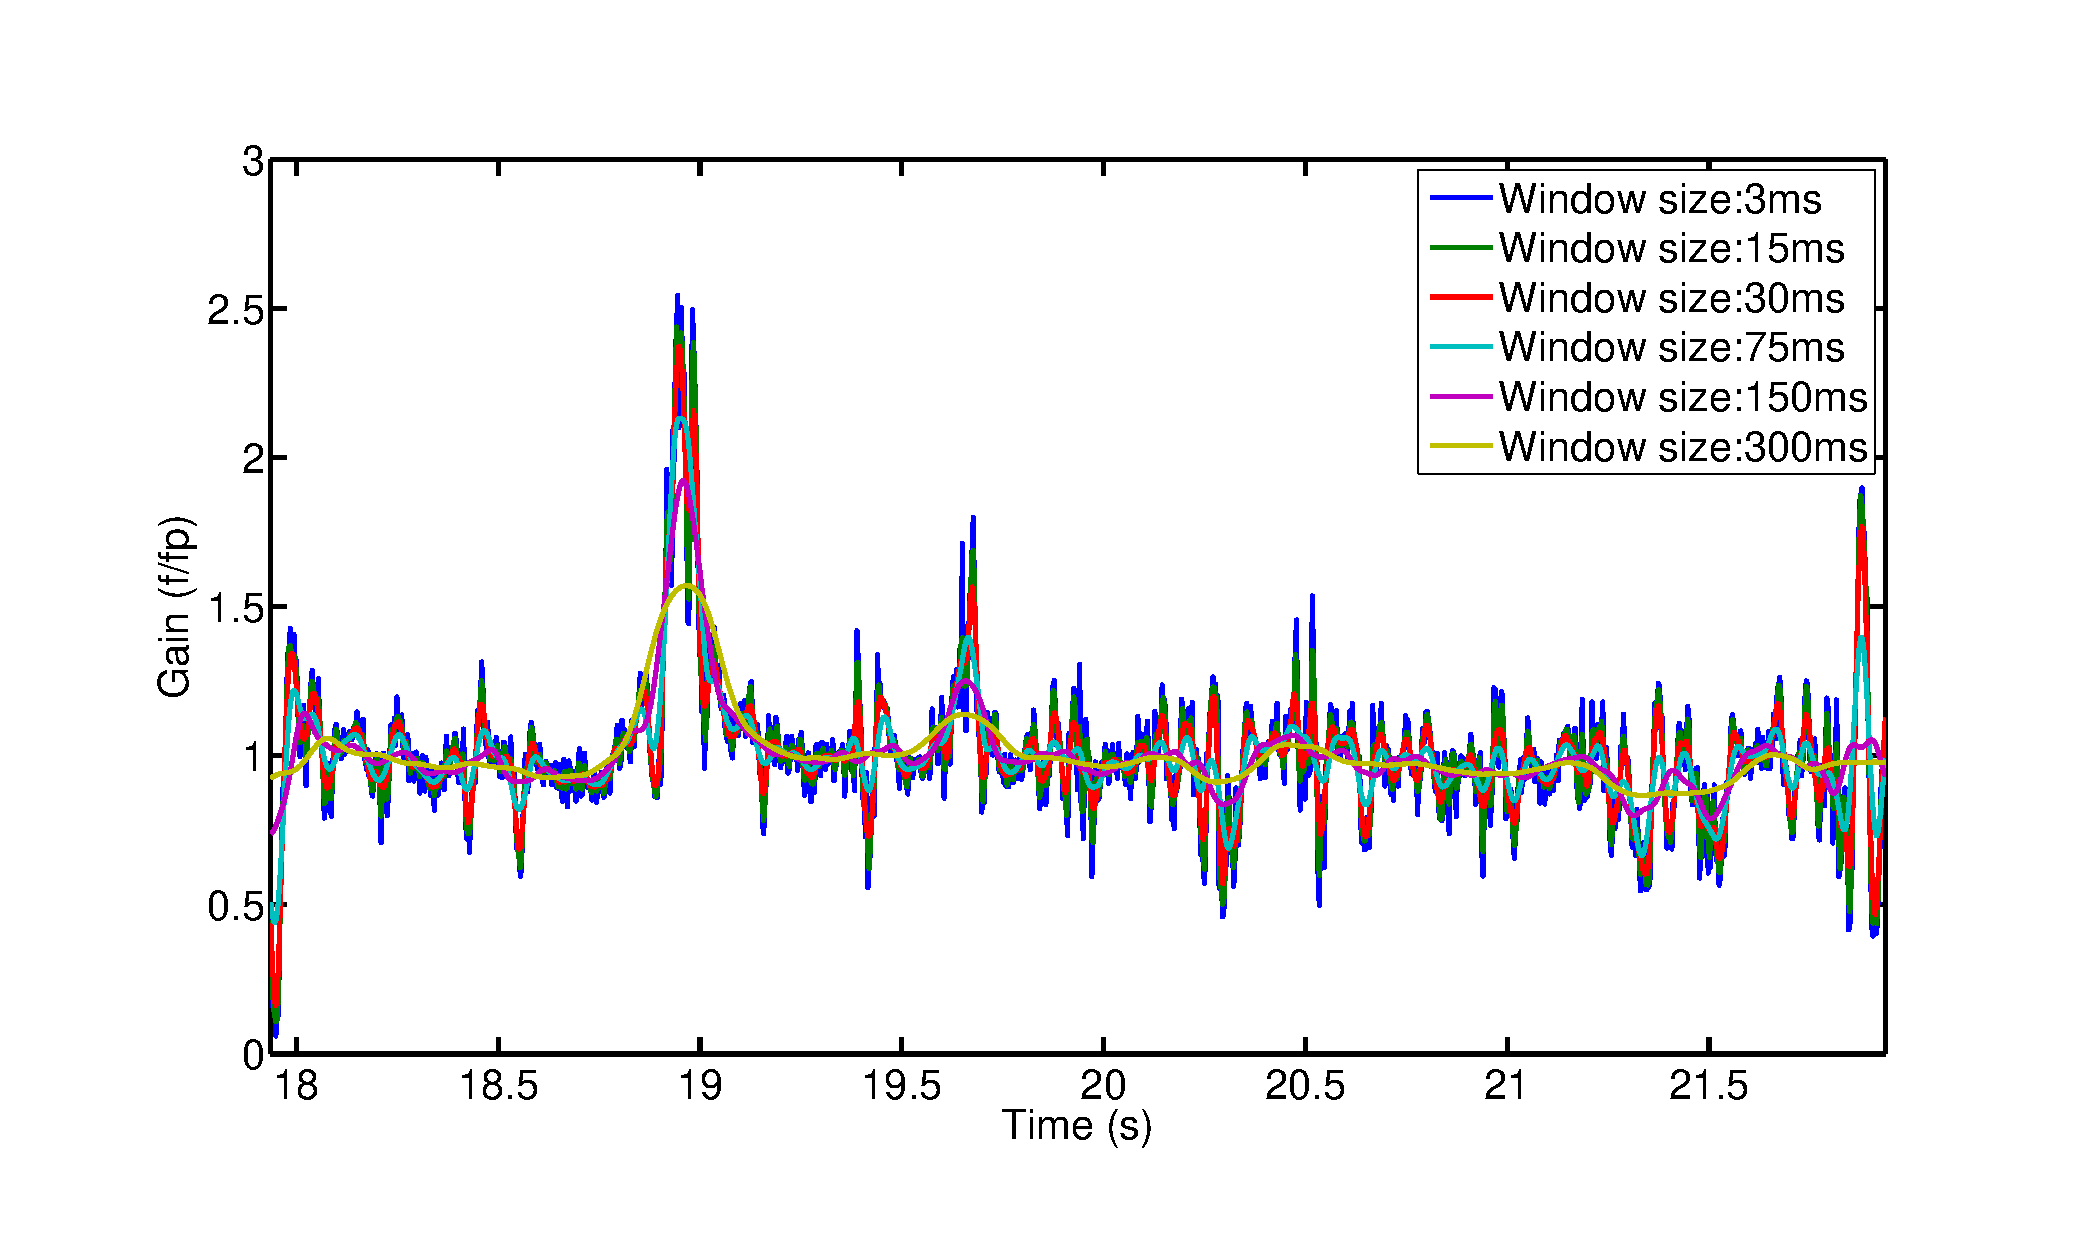
\includegraphics [width=\textwidth]{Analysis_January_21.pdf}
\begin{par}
The r-square of the smoothed ORN response to the actual data is
\end{par} \vspace{1em}

        \color{lightgray} \begin{verbatim}    0.9846

\end{verbatim} \color{black}
    \begin{par}
and the r-square of the smoothed ORN response to the predicted smoothed data is
\end{par} \vspace{1em}

        \color{lightgray} \begin{verbatim}    0.9723

\end{verbatim} \color{black}
    \begin{par}
The smoothing operation should not interfere with the gain modulation we observe. Here, we repeat the gain analysis, but this time with the smoothed data and the smoothed prediction.
\end{par} \vspace{1em}

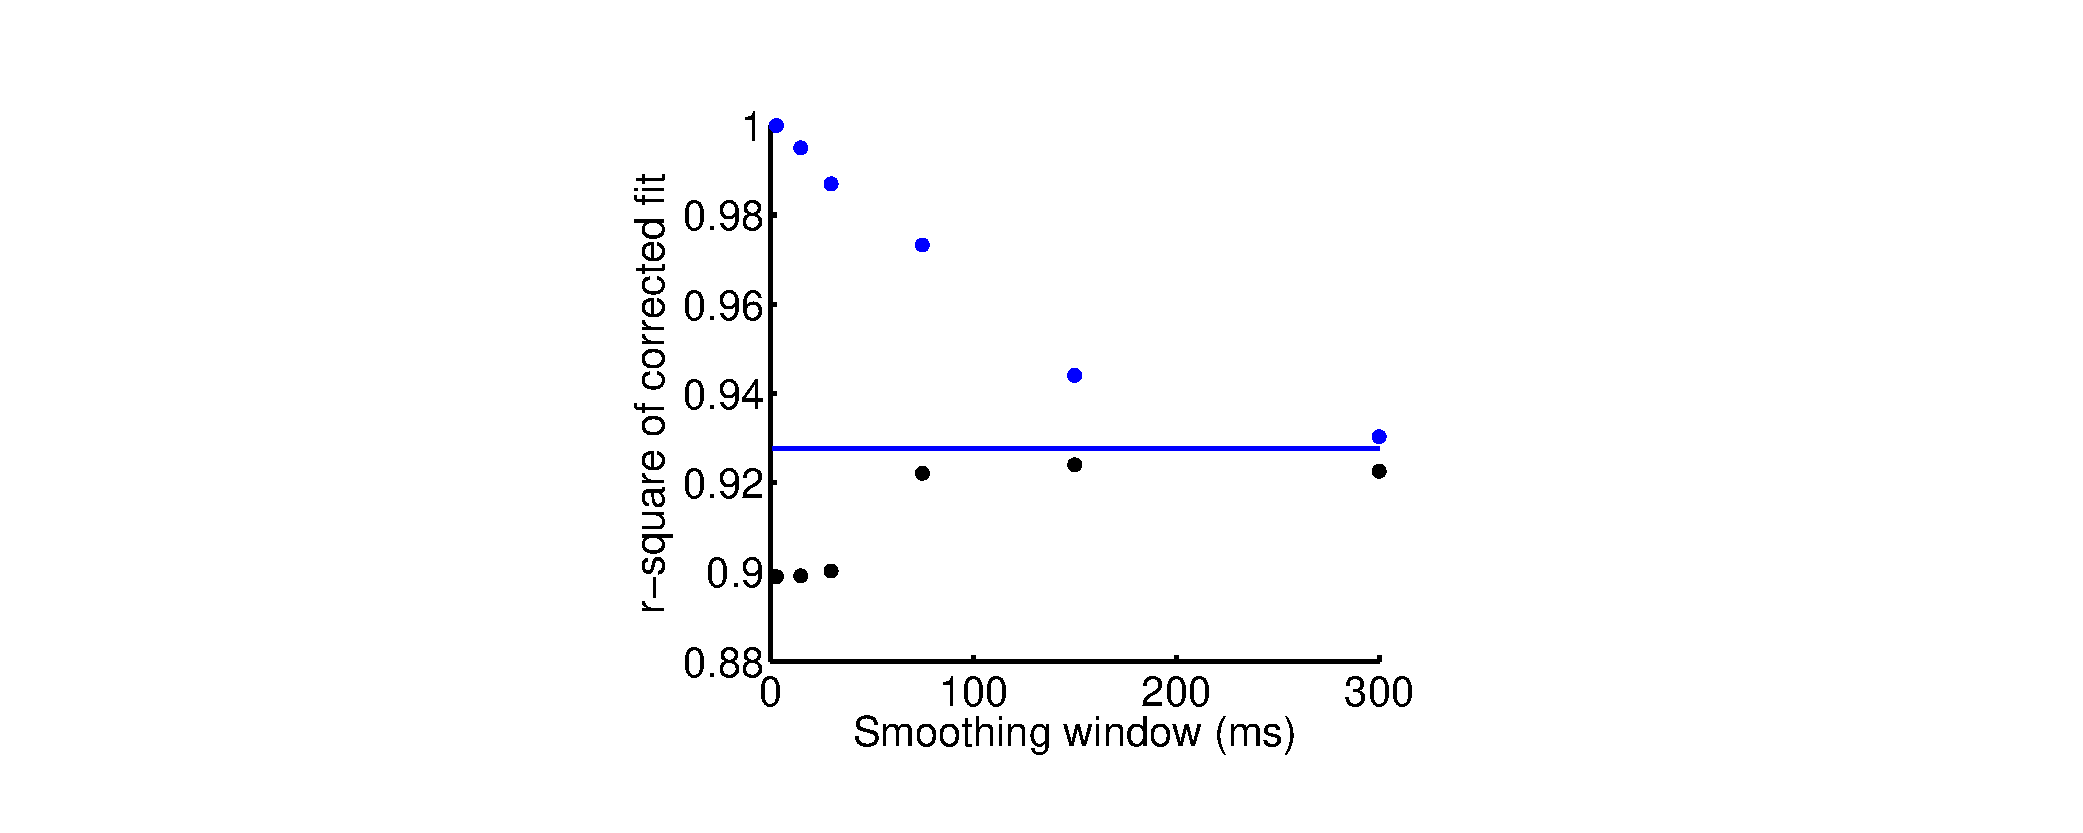
\includegraphics [width=\textwidth]{Analysis_January_22.pdf}
\begin{par}
Once again, we can estimate the instantaneous gain and construct a filter from the PID to the instantaneous gain. This filter looks like
\end{par} \vspace{1em}

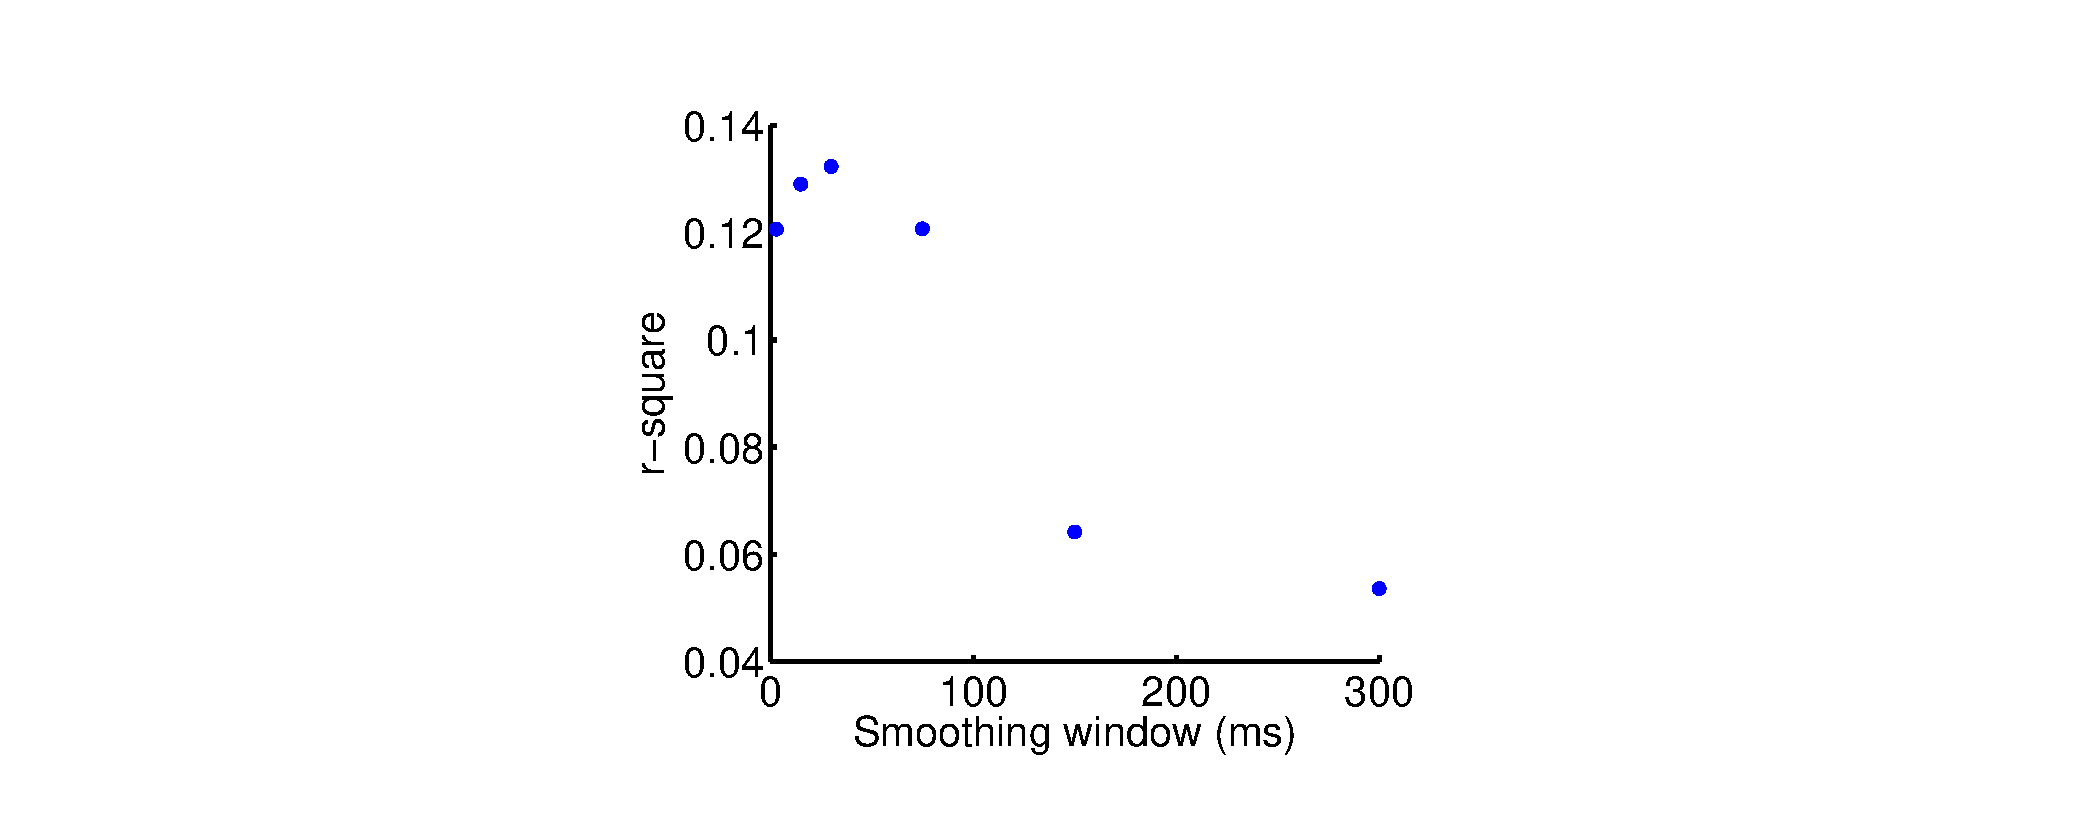
\includegraphics [width=\textwidth]{Analysis_January_23.pdf}
\begin{par}
This filter can be used to correct the simple linear prediction from the original data. Now, we can compare the gain-corrected prediction to the \textit{original unfiltered firing rate} and see if is better than the simple linear prediction.
\end{par} \vspace{1em}

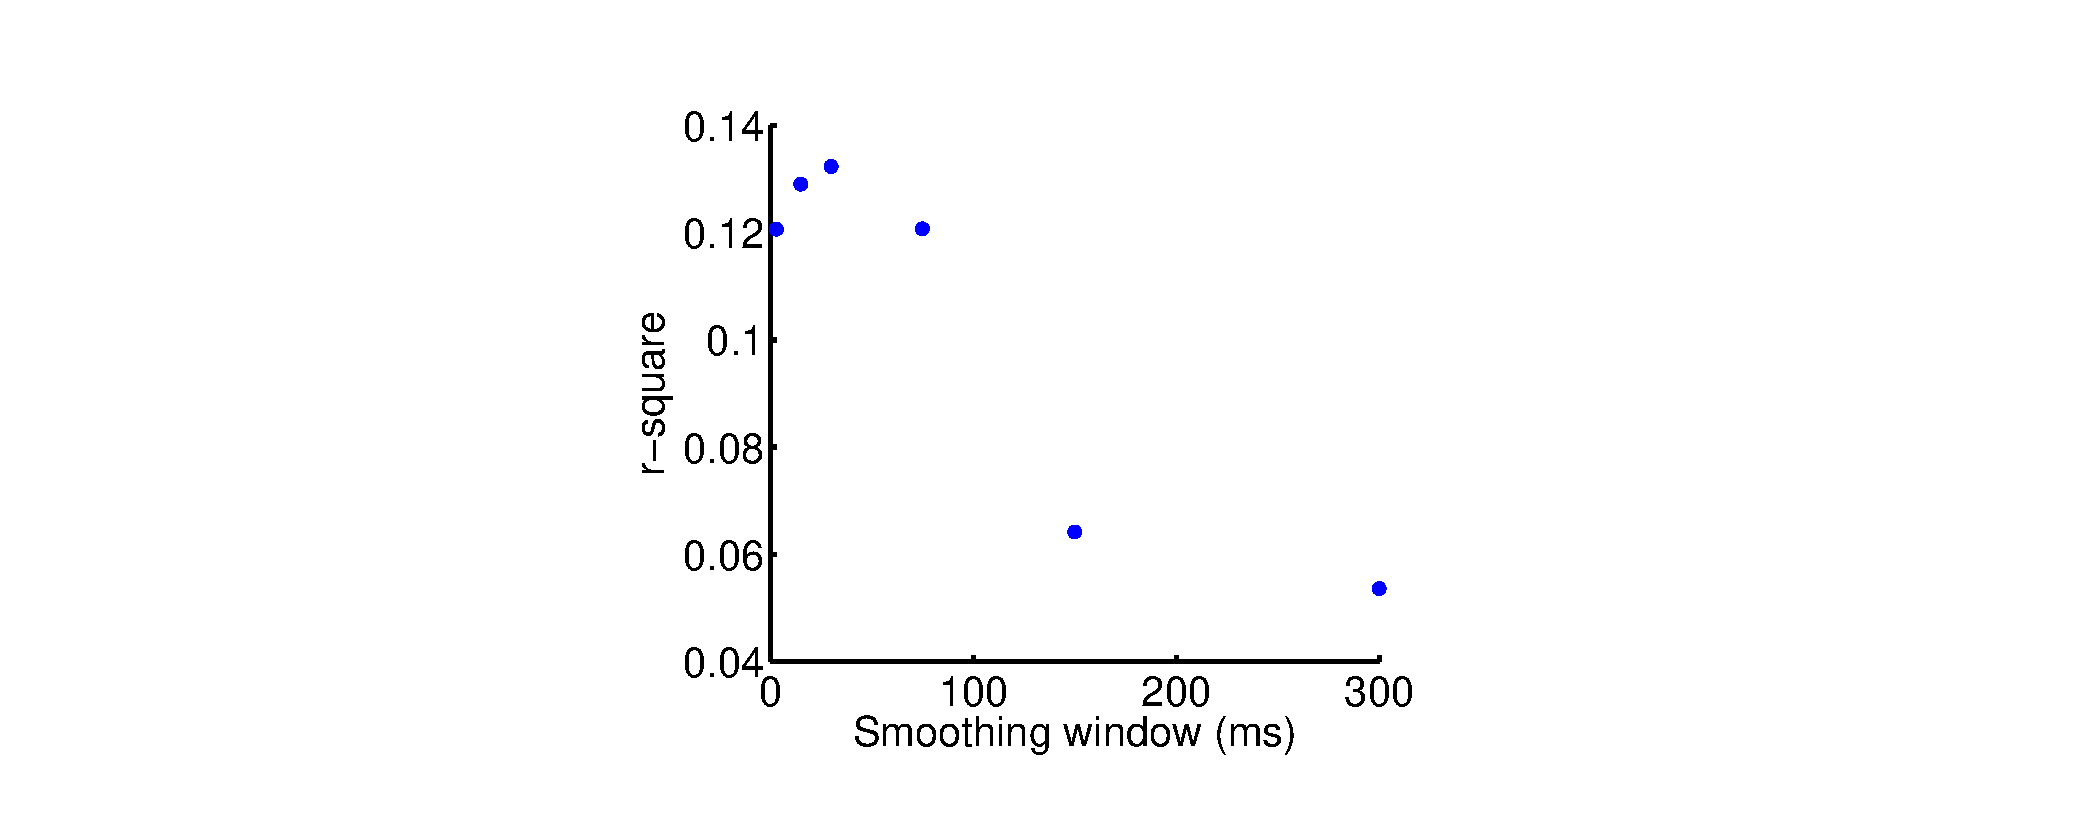
\includegraphics [width=\textwidth]{Analysis_January_24.pdf}
\begin{par}
The r-square of the gain-corrected prediction to the data is
\end{par} \vspace{1em}

        \color{lightgray} \begin{verbatim}    0.9616

\end{verbatim} \color{black}
    \begin{par}
\textit{cf.} the  r-square of the simple linear prediction to the data which is
\end{par} \vspace{1em}

        \color{lightgray} \begin{verbatim}    0.9592

\end{verbatim} \color{black}
    \begin{par}
Does this gain correction make the gains to low and high stimuli the same? In the following plot, we plot the best-fit lines of corrected prediction to data for different history lengths, and also show an example scatter plot for the gain corrected prediction.
\end{par} \vspace{1em}

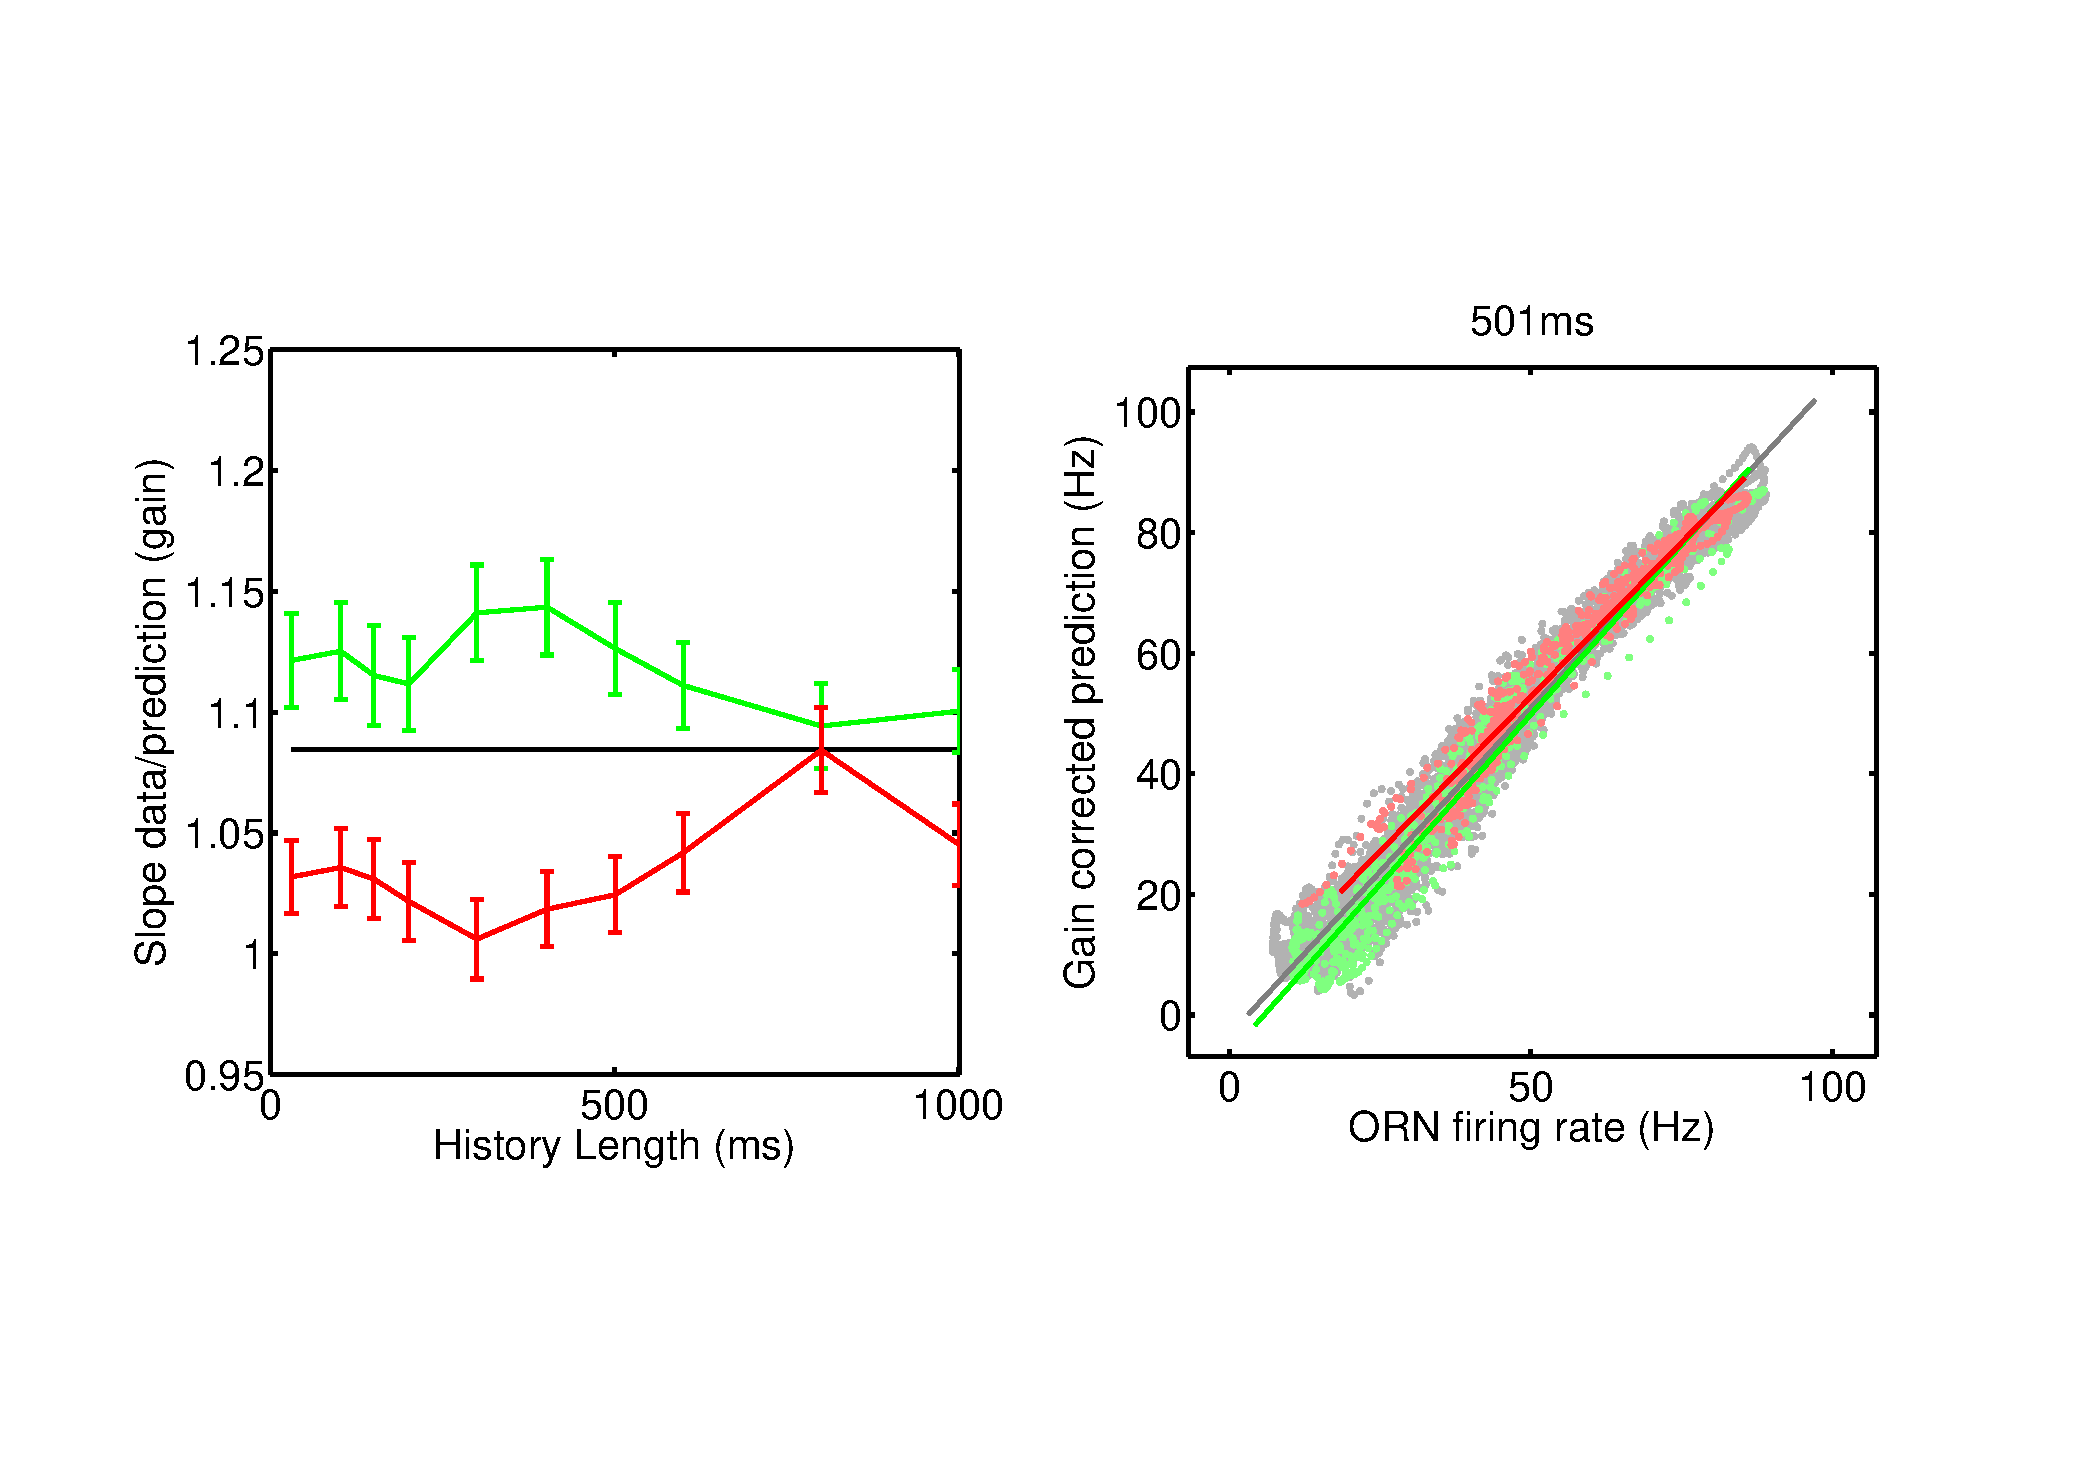
\includegraphics [width=\textwidth]{Analysis_January_25.pdf}


\subsection*{A note on elastic net regularisation}

\begin{par}
Carlotta says in her paper that she uses elastic net regularisation (using some unknown, third party code) to minimise the L-1 and L-2 norms of the covariance matrix. However, her code shows that she uses simply L-2 minimisation as discussed previously. I talked to her, and she said that she arbitrarily chose parameters for regularisation anyway, and it is possible that she was using simple L-2 regularisation, as this is a subcase of the elastic net regularisation.
\end{par} \vspace{1em}


\subsection*{Next Steps}

\begin{enumerate}
\setlength{\itemsep}{-1ex}
   \item Check if Weber's Law is being followed using Carlotta's step responses data
   \item Run analysis on all data files.
   \item Fit DA model to data with tau set to zero
\end{enumerate}


\subsection*{Docs}

\begin{par}
This document was generated by MATLAB's \textit{publish} function. All files needed to generate this document are on a git repository. To clone onto your machine, use:
\end{par} \vspace{1em}
\begin{verbatim}git clone https://srinivasgs@bitbucket.com/srinivasgs/da.git\end{verbatim}
\begin{par}
You will also need a bunch of functions that this depends on, which are also on git. Use
\end{par} \vspace{1em}
\begin{verbatim}git clone https://srinivasgs@bitbucket.com/srinivasgs/core.git\end{verbatim}
\begin{par}
to get these.
\end{par} \vspace{1em}
\begin{par}
Once you have everything, run these commands to generate this document:
\end{par} \vspace{1em}


\subsection*{MATLAB� Code}

\begin{verbatim}options = struct('showCode',false,'format','latex','imageFormat',...
'pdf','figureSnapMethod','print','stylesheet','srinivas_latex.xsl');
publish2('Analysis_January.m',options);\end{verbatim}



\end{document}
    
